% !TEX TS-program = pdflatex
% !TEX encoding = IsoLatin

\documentclass[a4paper,11pt,twoside,english]{toptesi}
\usepackage[latin1]{inputenc}
\usepackage[T1]{fontenc}
\usepackage{lmodern}
\usepackage[a-1b]{pdfx}
\usepackage{hyperref}
\usepackage{cite}
\usepackage{listings}
\usepackage{color}
\usepackage{url}
\usepackage{multirow}
\usepackage{amsmath}
\usepackage{verbatim}
\usepackage{amssymb}
\usepackage{pgfplots}
\usepackage{caption}
\usepackage{subcaption}
\usetikzlibrary{shapes.geometric, arrows, positioning}
\tikzstyle{process} = [rectangle, rounded corners, minimum width=3cm, minimum height=1.2cm, draw=black, fill=blue!20, text centered]
\tikzstyle{arrow} = [thick,->,>=stealth]
\tikzstyle{susceptible} = [circle, minimum size=1.2cm, draw=blue, fill=blue!20, text centered]
\tikzstyle{infected} = [circle, minimum size=1.2cm, draw=red, fill=red!20, text centered]
\tikzstyle{recovered} = [circle, minimum size=1.2cm, draw=green, fill=green!20, text centered]
\tikzstyle{arrow} = [thick,->,>=stealth]
\tikzstyle{compartment} = [rectangle, rounded corners, minimum width=2.5cm, minimum height=1.5cm, text centered, draw=black, fill=blue!20]
\tikzstyle{arrow} = [thick,->,>=stealth]
\tikzset{
	state/.style={circle, minimum size=1.2cm, draw=blue, fill=blue!20, text centered},
	arrow/.style={thick,->,>=stealth}
}
% Definition of a new language for listings
%\lstdefinelanguage{P4}
%{
%	% list of keywords
%	alsoletter=\#,
%	morekeywords={
%		header\_type,
%		fields,
%		header,
%		parser,
%		extract,
%		return,
%		default,
%		next,
%		\#define,
%		latest,
%		select,
%		apply,
%		control,
%		table,
%		reads,
%		actions,
%		modify\_field,
%		action,
%		valid,
%		nop,
%		exact,
%		lpm,
%		if,
%		hit,
%		and,
%		extern,
%		void,
%		bit
%	},
%	sensitive=true, % keywords are not case-sensitive
%	morecomment=[l]{//}, % l is for line comment
%	morecomment=[s]{/*}{*/}, % s is for start and end delimiter
%	morestring=[b]" % defines that strings are enclosed in double quotes
%}
%
%\definecolor{eclipseBlue}{RGB}{42,0.0,255}
%\definecolor{eclipseGreen}{RGB}{63,127,95}
%\definecolor{eclipsePurple}{RGB}{127,0,85}
%
%\lstset{
%	language={P4},
%	basicstyle=\fontsize{8}{9}\ttfamily, % Global Code Style
%	captionpos=b, % Position of the Caption (t for top, b for bottom)
%	extendedchars=true, % Allows 256 instead of 128 ASCII characters
%	tabsize=2, % number of spaces indented when discovering a tab 
%	columns=fixed, % make all characters equal width
%	keepspaces=true, % does not ignore spaces to fit width, convert tabs to spaces
%	showstringspaces=false, % lets spaces in strings appear as real spaces
%	breaklines=true, % wrap lines if they don't fit
%	frame=trbl, % draw a frame at the top, right, left and bottom of the listing
%	%frameround=tttt, % make the frame round at all four corners
%	framesep=4pt, % quarter circle size of the round corners
%	numbers=left, % show line numbers at the left
%	numberstyle=\tiny\ttfamily, % style of the line numbers
%	commentstyle=\color{eclipseGreen}, % style of comments
%	keywordstyle=\color{eclipsePurple}, % style of keywords
%	stringstyle=\color{eclipseBlue}, % style of strings
%}

\hypersetup{%
    pdfpagemode={UseOutlines},
    bookmarksopen,
    pdfstartview={FitH},
    colorlinks,
    linkcolor={blue},
    citecolor={blue},
    urlcolor={blue}
  }

\newtheorem{osservazione}{Osservazione}% Standard LaTeX
\newtheorem{definition}{Definition}


\begin{document}
\english

\ateneo{Politecnico di Torino}
\corsodilaurea{Mathematical Engineering}

\titolo{Modeling the new flu wave using data science and complex networks theory.}

\candidato{Francesco \textsc{Celino}}
\relatore{Prof.\ Lorenzo \textsc{Zino}}
\secondorelatore{Prof.\ Alessandro \textsc{Rizzo}}
\sedutadilaurea{\textsc{Academic~Year} 2024-2025}
\logosede{Cover/polito_new-1}


\CorsoDiLaureaIn{Master Degree course in\space}
\TesiDiLaurea{Master's Degree Thesis}
\InName{in}
\CandidateName{Candidate}
\AdvisorName{Supervisors}


\frontespizio % make cover page

\ringraziamenti

Ancora da fare...

\abstract
This Master's thesis explores how the SEINR (Susceptible, Exposed, Infectious, Non-infectious, Recovered) compartmental model can be used to forecast the evolution of influenza-like illness (ILI) cases in Italy during the 2023-24 winter season. The model's innovative aspects lie in its community-based meta-population framework, which simulates \textit{intra-} and \textit{inter-}regional mobility, capturing network dynamics critical to understanding how a disease spreads in Italy's diverse demographic and geographic landscape. This approach, which was previously successful when evaluating the efficacy of NPIs (non-pharmaceutical interventions) during the \textit{COVID-19} pandemic, is then further refined by taking into account features such as class divisions according to age, activity levels, and vulnerability to disease of different age groups, increasing the adaptability of the model to the Italian landscape.


Bayesian inference tools and Monte Carlo methods are then used to improve the estimates of a few fundamental epidemiological parameters such as transmission rate and infection duration. Our empirical results demonstrate the model's effectiveness in capturing flu trends in Italy.


This work emphasizes the role of adaptive modeling in epidemiology, and how public health strategies driven by past data can help in managing seasonal epidemics. 

\indici
\listoffigures
\listoftables
\mainmatter

\chapter{Introduction}
Each year, Influenza affects millions of people across the world, posing great challenges for healthcare systems in various developed countries, with great risks for elderly and more vulnerable people. In response, researchers and public health officials work to predict and control the spread of these diseases, using various tools and methods. One of the most powerful tools we have available is mathematical modeling, which allows us to simulate how a disease might spread through a population through the use of "differential equations". This thesis focuses on adopting one of such models\cite{par21} for flu-like illnesses in Italy, using a framework called the SEINR model.


The SEINR model is a type of "compartment" model. This means that it divides the population into different groups (or compartments) of people, based on the stages of the disease and whether or not they are infected. In this case, the compartments are \textit{Susceptible} (people who can catch the flu), \textit{Exposed} (people who have been infected but are not yet contagious), \textit{Infectious} (people who can spread the flu), \textit{Non-infectious} (people who do not present any symptom, or are isolated), and \textit{Removed} (people who are either immune to the flu after recovering, or dead due to complications). 


The history of compartmental models dates back to 1927, when Kermack and McKendrick\cite{ker27} defined the SIR model for the first time, in its simplest form. 


However, what makes the model we used for this thesis particularly innovative is its "meta-population" structure, already used with great success in 2021 when trying to model the first Covid-19 wave in Italy \cite{par21}. Instead of treating Italy as one large group of people, the meta-population approach breaks it down into regions and even considers how people move between these regions. This is crucial for a country like Italy, where people frequently travel between cities and regions for work, school, and other reasons. 


Most importantly, when trying to predict the outcomes of a Influenza season, we need to consider other crucial factors, such as vaccines, the age and activity levels of individuals, as well as their vulnerability to illness. These factors are important because some groups, like the elderly or those with pre-existing health conditions, are more at risk during a flu outbreak, but could very well be less exposed to the disease due to having less social contacts. If we want our predictions to be accurate, we need to take into account all of those factors. 


Another key feature of this thesis is the use of "Bayesian inference", a statistical method that allows the model to improve its accuracy (and precision) over time. As new weekly data about flu cases becomes available, the model updates its parameters in a probabilistic fashion: that means, if in one particular week we observe more infected people than we would expect, we probably need to rethink our predictions. That's why, when using Bayesian inference, we do not provide exact estimates for the number of infected people we will have next week, but rather a "probability distribution" that includes reasonable confidence intervals: as more weeks pass and we gather more real data, we expect those probability distributions to get narrower, reflecting our increased confidence on the disease's characteristics. 


In short, the goal of my thesis is to provide a more accurate and flexible tool for predicting flu-like illnesses in Italy, one that can adapt to different variants of Influenza each year (as you probably know, each year the flu outbreak is slightly different due to changing vaccines, mobility patterns, timing and public awareness). This tool can help public health officials better prepare for and respond to outbreaks, reducing the strain on healthcare systems and, who knows, maybe also save some lives. 


I am also proud to say that, thanks to the invaluable guidance of my supervisors, we were able to use this model to contribute to two major forecasting projects at the European level. Through these projects, I had the opportunity to collaborate with the \textit{ISI Foundation} and the \textit{Istituto Superiore di Sanita'}, as we provided weekly estimates for the evolution of last year's flu season.

\cite{par21}

%\section{Plagiarism}

%To be approved, your thesis must pass a plagiarism check. As a reminder:
%\begin{itemize}
%\item it is forbidden to copy verbatim one or more sentences  from any other external source (web pages, papers, etc.), unless you explicitly  grant the source and put the sentence/sentences in ``...''. Your can instead rephrase the whole sentence/sentences.
%\item it is forbidden to include an image (diagram or figure) taken from web pages or papers. It is better to redraw. If you really need to include  an image from an external source, you must add to the caption ``(Reproduced from~\cite{example})'', citing properly the source.
%\end{itemize}

 
\chapter{Methods}
The framework which will be used in this project is the one outlined by compartmental models, which aim to divide a population into distinct groups, or compartments, based on their status in relation to the disease. These models provide a simplified yet powerful way to describe the progression of an epidemic through a population using systems of ordinary differential equations (ODEs), in which each variable represents a compartment, and each parameter is modelled according to biological inferences. 

The earliest modern compartmental model is the SIR model, introduced by Kermack and McKendrick in 1927 \cite{ker27}. As implied by the name, the SIR model divides the population into three compartments: \textit{Susceptible} (S), representing individuals who can contract the disease; \textit{Infectious} (I), representing those actively spreading the disease; and \textit{Removed} (R), which includes individuals who have recovered and gained immunity or have died. The dynamics of the SIR model are governed by the following system of ODEs:

\begin{equation}
	\begin{aligned}
		\frac{dS}{dt} &= -\beta \frac{SI}{N}, \\
		\frac{dI}{dt} &= \beta \frac{SI}{N} - \gamma I, \\
		\frac{dR}{dt} &= \gamma I,
	\end{aligned}
\end{equation}

\begin{figure}[h]
	\centering
	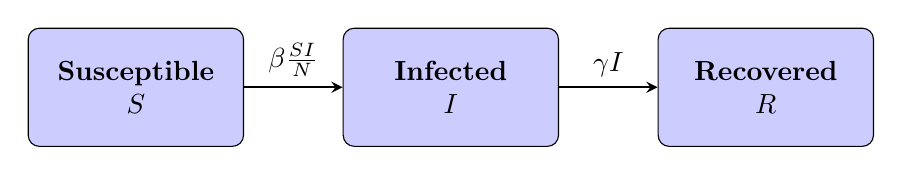
\begin{tikzpicture}[node distance=4cm]
		
		% Nodes (using \parbox to allow multi-line text)
		\node (S) [compartment] {\parbox{2.5cm}{\centering \textbf{Susceptible} \\ $S$}};
		\node (I) [compartment, right of=S] {\parbox{2.5cm}{\centering \textbf{Infected} \\ $I$}};
		\node (R) [compartment, right of=I] {\parbox{2.5cm}{\centering \textbf{Recovered} \\ $R$}};
		
		% Arrows with transition labels
		\draw [arrow] (S) -- (I) node[midway, above] {$\beta \frac{SI}{N}$};
		\draw [arrow] (I) -- (R) node[midway, above] {$\gamma I$};
		
	\end{tikzpicture}
	\caption{Flowchart of the SIR Compartmental Model.}
\end{figure}

where \(N\) is the total population size, \(\beta\) is the transmission rate, and \(\gamma\) is the recovery rate. It is apparent that one of the key hypotheses of the SIR model is that a person cannot become infectious twice: once that person has recovered, they cannot become susceptible again. The model also assumes that our total population remains constant over time: the total sum of $ S + I + R $ cannot change over time, and this fact is easily verifiable by integrating these equations with respect to time. 

This model's simplicity, while being its greatest strength, is also a major weakness: the model does not contemplate an "asymptomatic period" of sorts, since as soon as you are taken out of the susceptible compartment you can already spread the disease to other people. This behaviour does not describe real-life epidemic phenomena correctly, but makes the model simpler conceptually and easier-to-use. 

For my thesis, a more complex model was needed: building upon the SIR framework, the \textbf{SEINR model} introduces additional compartments to better capture the complexities of real-world epidemics. Specifically, the SEINR model includes:

\begin{itemize}
	\item \textbf{Susceptible (S):} Individuals who can contract the disease.
	\item \textbf{Exposed (E):} Individuals who have been infected but are not yet infectious, representing the incubation period.
	\item \textbf{Infectious (I):} Individuals who can transmit the disease.
	\item \textbf{Non-infectious (N):} Individuals who no longer spread the disease, either because they are isolated, mildly ill, or simply no longer symptomatic. 
	\item \textbf{Removed (R):} Individuals who have either recovered and gained immunity or succumbed to the disease.
\end{itemize}

The inclusion of the \textbf{Exposed} and \textbf{Non-infectious} compartments allows the SEINR model to more accurately reflect diseases with an incubation period or asymptomatic cases, which are common in influenza-like illnesses. The same hypotheses we made with the SIR model about the conservation of the population (no births or deaths unrelated to the disease) and the impossibility of becoming ill twice apply here. 

An important concept that arises in compartmental models with a \textbf{Removed} compartment is \textbf{herd immunity}. Herd immunity occurs when a sufficient portion of the population becomes immune, either through infection or vaccination, thereby reducing the probability of disease transmission to susceptible individuals. This phenomenon is closely related to the \textbf{basic reproduction number} (\(R_0\)), a constant that represents the average number of secondary infections generated by a single infectious individual in a fully susceptible population. In other words, if a disease has a basic reproduction number greater than one, that disease should theoretically spread indefinitely, since each person infects more than one person before recovering (on average). 

For simplicity's sake, let us consider the SIR model, where herd immunity is achieved when the fraction of the population that remains susceptible falls below a critical threshold, given by:

\begin{equation}
	S_c = \frac{1}{R_0}.
\end{equation}

At this point, the effective reproduction number (\(R_t = R_0 \cdot \frac{S}{N}\)) drops below 1, causing the epidemic to decline. This principle also holds true for more complex models like SEINR, where, as explained, the dynamics of immunity and disease spread are also influenced by latency periods and non-infectious stages. This behaviour is harder to describe in analitical terms, but will be numerically visible in the following experiments. 

\begin{figure}[h]
	\centering
	% First subplot: R_0 < 1 (infection dies out)
	\begin{subfigure}{0.45\textwidth}
		\centering
		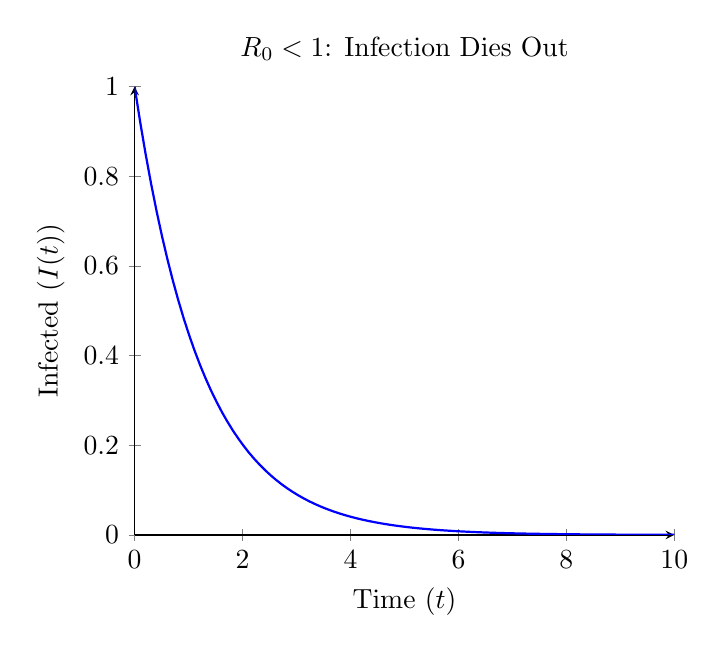
\begin{tikzpicture}
			\begin{axis}[
				domain=0:10,
				samples=100,
				xlabel={Time ($t$)},
				ylabel={Infected ($I(t)$)},
				title={$R_0 < 1$: Infection Dies Out},
				axis lines=left,
				ymin=0, ymax=1,
				xtick={0,2,4,6,8,10},
				ytick={0,0.2,0.4,0.6,0.8,1},
				every axis plot/.append style={thick}
				]
				% Exponential decay curve: infection fades out
				\addplot[blue] {exp(-0.8*x)};
			\end{axis}
		\end{tikzpicture}
	\end{subfigure}
	\hfill
	% Second subplot: R_0 > 1 (infection spreads)
	\begin{subfigure}{0.45\textwidth}
		\centering
		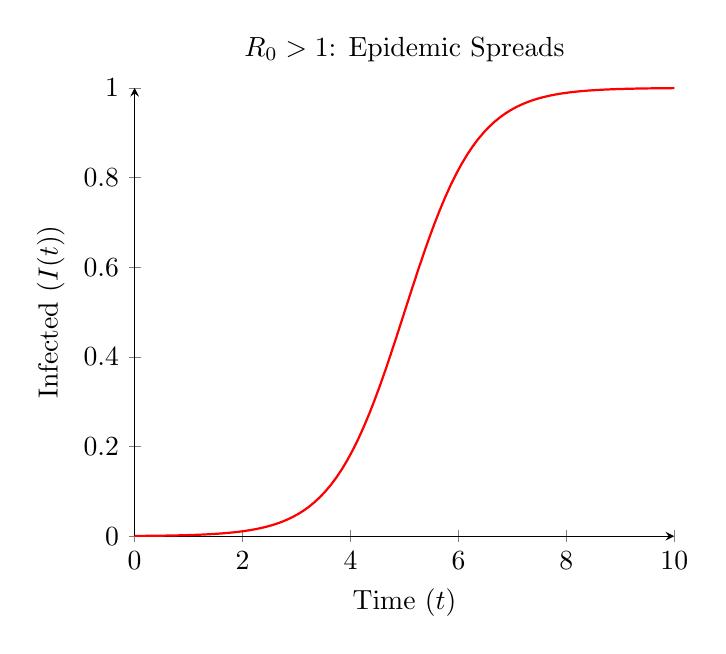
\begin{tikzpicture}
			\begin{axis}[
				domain=0:10,
				samples=100,
				xlabel={Time ($t$)},
				ylabel={Infected ($I(t)$)},
				title={$R_0 > 1$: Epidemic Spreads},
				axis lines=left,
				ymin=0, ymax=1,
				xtick={0,2,4,6,8,10},
				ytick={0,0.2,0.4,0.6,0.8,1},
				every axis plot/.append style={thick}
				]
				% Sigmoid-like curve: infection grows
				\addplot[red] {1/(1 + exp(-1.5*(x-5)))};
			\end{axis}
		\end{tikzpicture}
	\end{subfigure}
	
	\caption{Comparison of infection dynamics based on $R_0$. Left: If $R_0 < 1$, infection decreases and dies out. Right: If $R_0 > 1$, infection spreads and leads to an epidemic.}
\end{figure}

In the context of seasonal influenza, if we make the assumption that a person can only become infected once each year, the concept of herd immunity plays a significant role in shaping public health strategies, particularly in designing vaccination campaigns (many compartmental models automatically include vaccinated people in the removed compartment). By estimating \(R_0\) and tracking its progression as the epidemic goes on, one can gain insight into how contagious a certain virus or bacteria strain is in a certain place at a certain time, and thus whether implementing non-pharmaceutical interventions (NPIs), such as social distancing or lockdowns, is warranted. 

%Inizia parlando dei modelli a compartimenti in generale, introduci il SIR, parla della struttura a equazioni diff. alle derivate ordinarie, introduci il modello SEINR generale coi 5 diversi compartimenti. Parla del concetto di immunit� di gregge nei modelli col compartimento removed, in funzione del numero di riproduzione di base
 
\section{The Metapopulation SEINR Framework}

\subsection{Activity-Driven Meta-Population Model}

In the \textit{Metapopulation} framework, we partition a population of \(n\) individuals into \(K\) communities, denoted as \(\mathcal{H} = \{1, \ldots, K\}\): each community represents bounded and well-defined geographical areas (e.g., regions, provinces, or cities). Each community \(h \in \mathcal{H}\) contains \(n_h\) people. The way a community interacts with other communities in the model is described by a \textit{weighted graph}, where each edge represents a travel path. The weights of this graph are described using the \textit{routing matrix} \(\mathbf{W} \in [0,1]^{K \times K}\), which defines the fraction of individuals in a certain community that move to other communities when becoming "active". For example, \(\mathbf{W}_{hk}\) denotes the fraction of individuals from community \(h\) that travel to community \(k\) in a given time unit (as we will see, a time unit represents a day in our model). The matrix satisfies:
\[
\mathbf{W}_{hh} = 0, \quad \sum_{k=1}^K \mathbf{W}_{hk} = 1, \quad \forall h.
\]

The inhabitants of each community are then divided into \(P\) "activity classes", \(a_1, a_2, \ldots, a_P\), where \(0 < a_i \leq 1\). The baseline activity \(a_i\) quantifies the propensity of individuals in class \(i\) to interact with other people. At each time step, a fraction \(a_i\) of individuals in each class becomes active, either interacting "locally" or traveling to other communities as determined by the \textit{mobility parameter} \(b \in [0,1]\). This parameter simply represents the fraction of active individuals commuting to other communities (thus coming into contact with people from other communities), with the remaining \(1 - b\) interacting within their own community.

\subsection{Disease Progression}

As explained, the dynamics of the disease will be modeled using the susceptible--exposed--infectious--non-infectious--removed (SEINR) framework. After contagion, susceptible individuals move into the \textit{Exposed} (\(E\)) compartment with rate \(\lambda\), representing the latency period before becoming infectious. The transitions between compartments are defined as follows:
\begin{itemize}
	\item \(E \to I\): Transition to the \textit{Infectious} (\(I\)) compartment occurs at rate \(\nu\), with \(1/\nu\) representing the average latency period.
	\item \(I \to N\): Transition to the \textit{Non-infectious} (\(N\)) compartment occurs at rate \(\mu\), where \(1/\mu\) is the average infectious period.
	\item \(N \to R\): Transition to the \textit{Removed} (\(R\)) compartment occurs at rate \(\gamma\), while \(1/\gamma\) represents the average delay before recovery or death.
\end{itemize}

\begin{figure}[h]
	\centering
	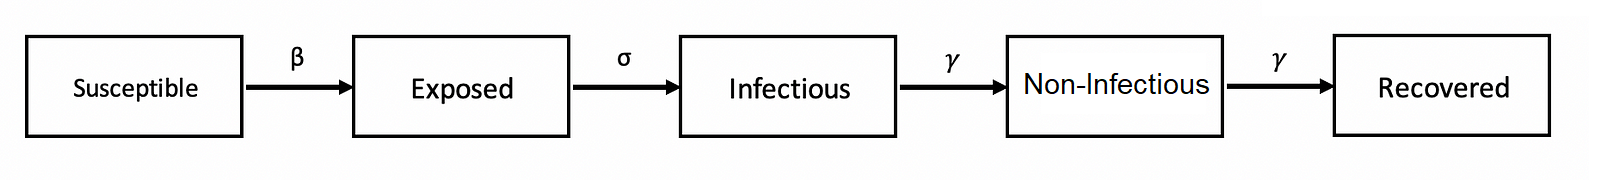
\includegraphics[width=0.7\textwidth]{Figures/SEINR.png}  % Replace with actual figure file
	\caption{A flow chart explaining how the SEINR compartmental model is organized}
	%\label{fig:commuting_matrix}
\end{figure}

It is clear that the average time from infectiousness to removal is \(1/\mu + 1/\gamma\). The transition between compartments is regulated by the following set of ODEs:
\[
\begin{aligned}
	S_i^h(t+1) &= \big(1 - \Pi_i^h(t)\big) S_i^h(t), \\
	E_i^h(t+1) &= \Pi_i^h(t) S_i^h(t) + \big(1 - \nu\big) E_i^h(t), \\
	I_i^h(t+1) &= \nu E_i^h(t) + \big(1 - \mu\big) I_i^h(t), \\
	N_i^h(t+1) &= \mu I_i^h(t) + \big(1 - \gamma\big) N_i^h(t).
\end{aligned}
\]

Where \(\Pi_i^h(t)\) represents the contagion probability, which will be defined in the following section. 
\subsection{Contagion Mechanism and Contact Probabilities}

If an infectious person comes into contact with a susceptible person, the latter will not always become infected. This uncertainty is captured by the probability of contagion, \(\Pi_i^h(t)\), represents the fraction of susceptible individuals in activity class \(i\) in community \(h\) that transition to the \(E\) compartment due to an interaction with infectious individuals. Since we are dealing with large populations, we can assume a thermodynamic limit (\(n \to \infty\)) and low epidemic prevalence (as we will see, this is in line with real-life data), and \(\Pi_i^h(t)\) can be expressed as:
\[
\Pi_i^h(t) = m \alpha a_i (1 - \beta b) \lambda P_h + m (1 - \alpha \beta a_i b) \lambda Q_h + m \alpha \beta a_i b \sum_{k \in \mathcal{H}} \mathbf{W}_{hk} \lambda P_k + m \alpha \beta a_i b \sum_{k \in \mathcal{H}} \mathbf{W}_{hk} \lambda Q_k,
\]
where:
\[
P_h = \frac{1}{\tilde{n}_h} \left( \sum_{j=1}^P (1 - \alpha \beta a_j b) I_j^h + \sum_{k \in \mathcal{H}} \mathbf{W}_{hk} \sum_{j=1}^P \alpha \beta a_j b I_j^k \right),
\]
\[
Q_h = \frac{1}{\tilde{n}_h} \left( \sum_{j=1}^P (1 - \beta b) \alpha a_j I_j^k + \sum_{k \in \mathcal{H}} \mathbf{W}_{hk} \sum_{j=1}^P \alpha \beta a_j b I_j^k \right),
\]
and \(\tilde{n}_h\), is the effective population size in community \(h\). This is defined as

\begin{figure}[h]
	\centering
	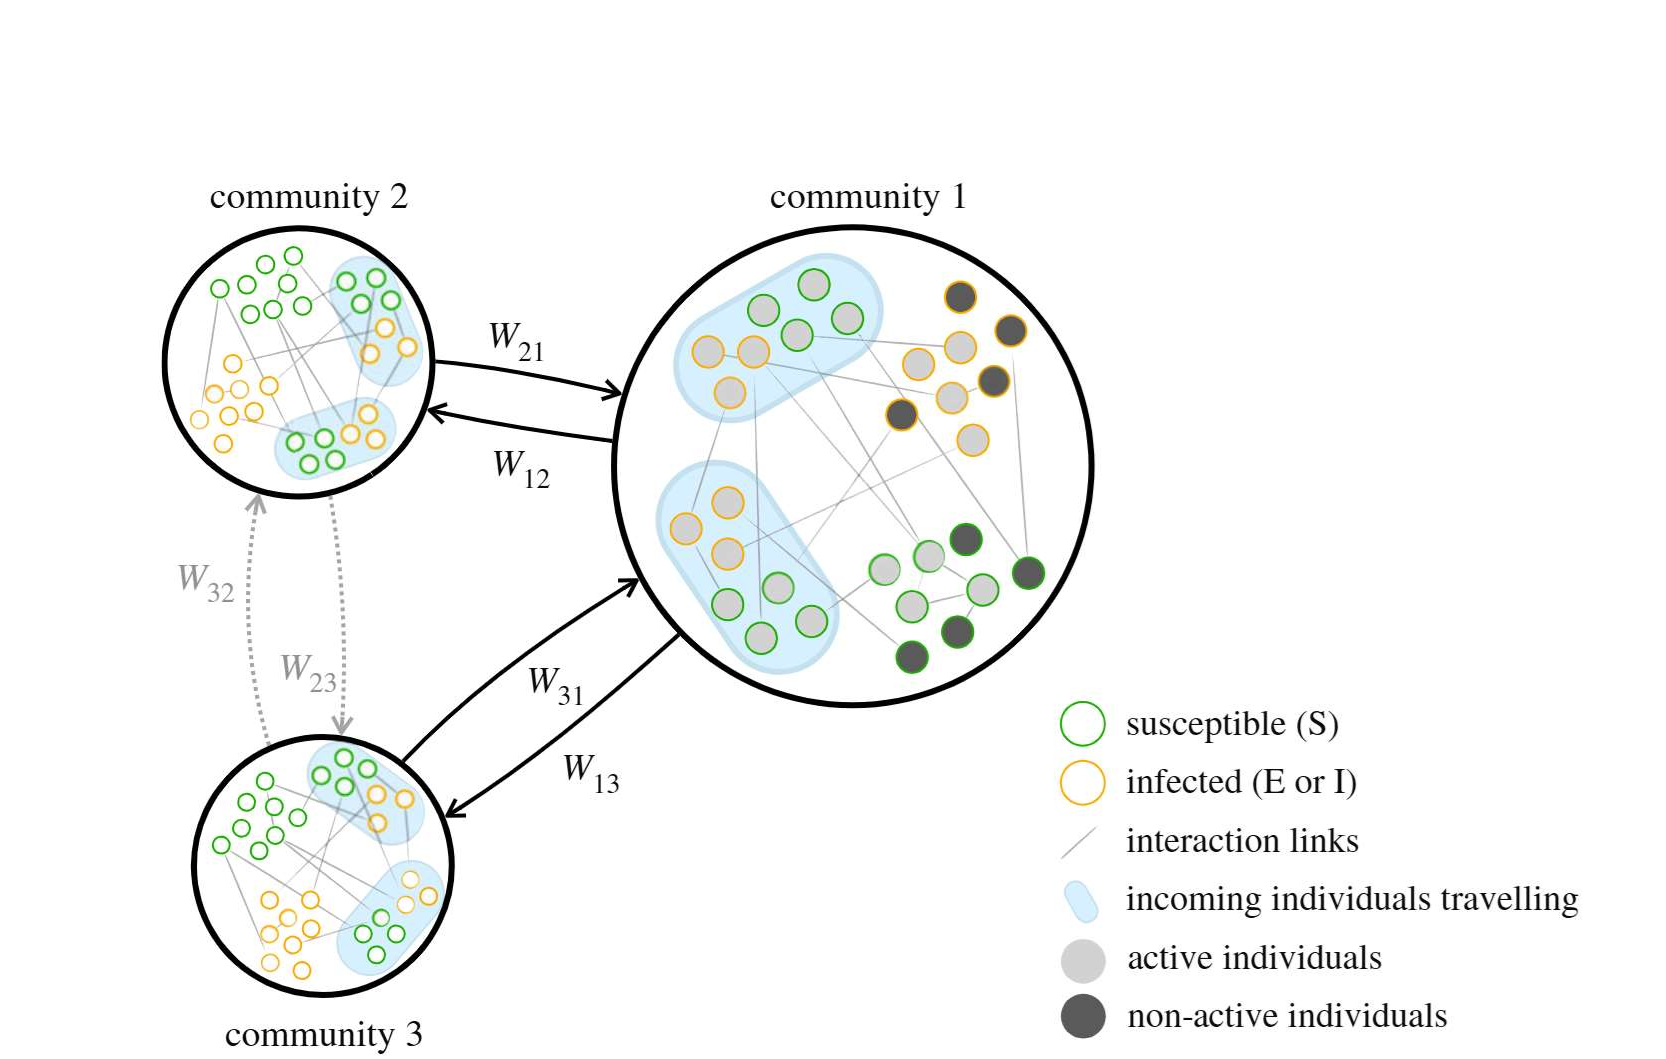
\includegraphics[width=0.7\textwidth]{Figures/communities_interaction.png}  % Replace with actual figure file
	\caption{Interactions between communities in the Metapopulation framework. Taken from \cite{par21}}
	%\label{fig:commuting_matrix}
\end{figure}

Thus, we now have a SEINR framework that incorporates interactions between various communities.

%Spiega cosa c'e' di nuovo nell'approccio a meta-popolazione, come funzionano i contatti fra individui, come ci si sposta. Spiega cos'e' una matrice di pendolarismo, e come si calcolano le probabilit� di contatto. 

\subsection{Age classes}
Some age brackets, such as the elderly, tend to have fewer social interactions compared to younger people. However, they also have a significantly higher probability of developing severe complications in case of infection. 

To account for this, the population was partitioned in 2 age classes, the former of which contains every individual who is less than 65 years old, and the latter includes everyone else. The fraction of individuals in each age classes was calibrated using italian census data\cite{istat}. 

\subsection{Commuting matrix}
The commuting matrix is estimated using official census data\cite{istat}. Each entry \(W_{hk}\) of the matrix denotes the proportion of individuals from region \(h\) that commute to region \(k\). The structure of the commuting matrix significantly influences disease spread since regions with high incoming mobility may experience faster outbreaks due to external infections. 

Figure~\ref{fig:commuting_matrix} illustrates the structure of the commuting matrix used in our model.

\begin{figure}[h]
	\centering
	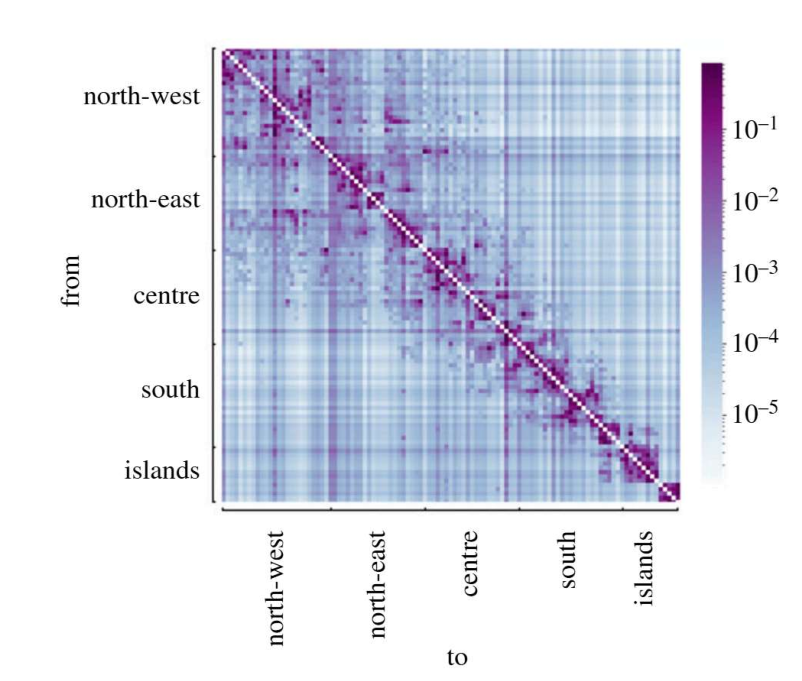
\includegraphics[width=0.7\textwidth]{Figures/commuting_matrix.png}  % Replace with actual figure file
	\caption{Representation of the commuting matrix \(W\) showing mobility patterns between different regions. Taken from \cite{par21}}
	\label{fig:commuting_matrix}
\end{figure}

\subsection{Vaccines}

In Italy, about two-thirds of the elderly population becomes vaccinated against Influenza each year, with the vaccination campaign typically occurring between October and December \cite{vaxita23}. 

To integrate the concept of vaccination in our model, we created a new class for \textit{vaccinated elderly} people (with its own activity level $a_elderly$), in addition to the existing classes for the general elderly and young populations. The transition from the \textit{elderly} class to the \textit{vaccinated elderly} class occurs instantaneously once a predefined threshold date is reached, as an approximation of the timing of the real-world vaccination campaign.

Vaccine efficacy values are taken from \cite{vax23} and are applied to reduce the probability of transition from the \textit{susceptible} to the \textit{exposed} compartment. This adjustment reflects the protective effect of vaccination against infection. In addition to that, vaccinated individuals retain a lower probability of developing severe complications, in line with empirical data on vaccine effectiveness.
 
\section{Other parameters}
\begin{table}[h]
	\centering
	\renewcommand{\arraystretch}{1.2}
	\begin{tabular}{|l|c|l|}
		\hline
		\textbf{Meaning} & \textbf{Value(s)} & \textbf{Reference} \\
		\hline
		$1/\nu$ & Latency period & \\
		$1/\mu$ & Infectiousness period & \\
		$1/\gamma$ & Time from infectiousness to reported death & \\
		$\lambda$ & Per-contact infection probability & $\surd$ \\ 
		$\eta$ & Class distribution & \\
		$a$ & Baseline activity & \\
		$b$ & Mobility parameter & \\
		$\alpha_{\text{low}}$ & Activity reduction & $\surd$ \\
		$m$ & Average number of contacts & \\
		$\beta_{\text{low}}$ & Mobility reduction & $\surd$ \\
		\hline
	\end{tabular}
	\caption{Summary of additional model parameters.}
	\label{tab:parameters}
\end{table}


\section{Real-world Data}

In order to validate our model, it is necessary to rely on real-world epidemiological data: in our case, we decided to utilize the weekly incidence of influenza-like illnesses (ILI) at the regional level. These data are sourced from the official \textit{Influcast} project repository on GitHub \cite{github}, which provides up-to-date weekly reports on influenza incidence across Italian regions. These data are publicly available, and the information provided has its roots in a network of Italian doctors that decided to contribute to the \textit{Influcast} project by sending data about how many of their patients show signs of flu illness. \begin{figure}[h]
	\centering
	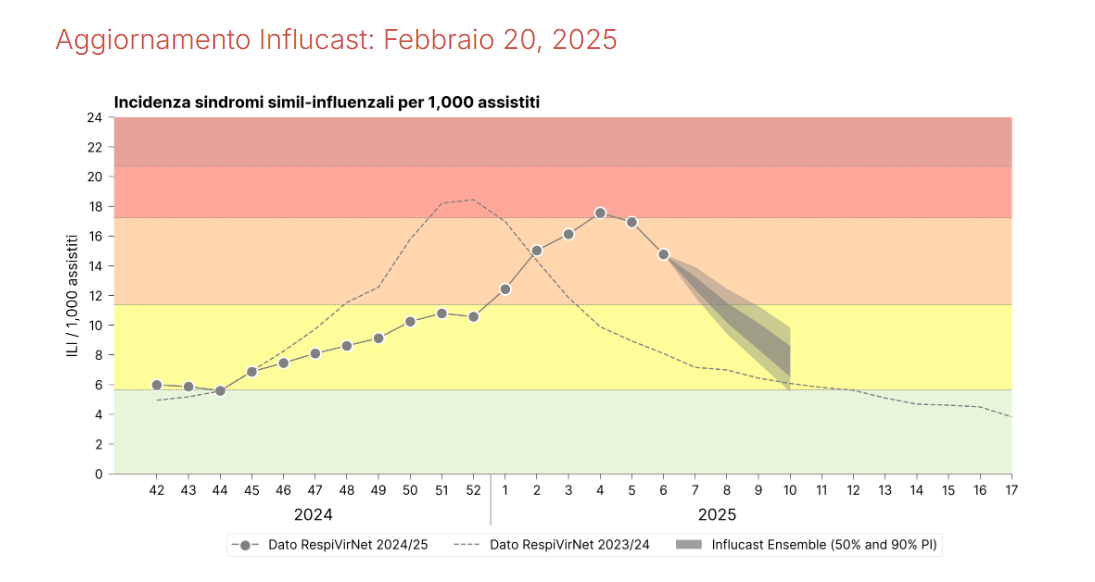
\includegraphics[width=0.7\textwidth]{Figures/incidence_time_series.png}  % Replace with actual figure file
	\caption{Incidence as a function of week number for various years. Taken from \cite{insight}}
	%\label{fig:commuting_matrix}
\end{figure}



\subsection{Data Format}

The data are provided as CSV files, where each row represents the recorded incidence for a specific week in a given region. Each file (for example \textit{marche-2023-52-ILI.csv} has the following format):
\begin{itemize}
	\item \textbf{Year} (\texttt{anno}): The calendar year of the observation.
	\item \textbf{Week} (\texttt{settimana}): The calendar week number.
	\item \textbf{Number of Cases} (\texttt{numero\_casi}): The number of reported ILI cases in the region by the surveillance system.
	\item \textbf{Number of Assisted Individuals} (\texttt{numero\_assistiti}): The total number of patients monitored by the surveillance system.
	\item \textbf{Incidence} (\texttt{incidenza}): The estimated incidence per 1000 inhabitants (in our case, this is simply the number of cases divided by the total number of monitored people times 1000).
	\item \textbf{Target} (\texttt{target}): The type of disease being monitored (ILI, in this case).
\end{itemize}

Table~\ref{tab:csv_format} shows an example of this structure:

\begin{table}[h]
	\centering
	\renewcommand{\arraystretch}{1.2}
	\begin{tabular}{|c|c|c|c|c|c|}
		\hline
		\textbf{Year} & \textbf{Week} & \textbf{Cases} & \textbf{Assisted} & \textbf{Incidence} & \textbf{Target} \\
		\hline
		2023 & 45 & 137.0 & 24447.0 & 5.6 & ILI \\
		2023 & 46 & 197.0 & 29651.0 & 6.64 & ILI \\
		2023 & 47 & 216.0 & 33744.0 & 6.4 & ILI \\
		2023 & 48 & 335.0 & 36037.0 & 9.3 & ILI \\
		2023 & 49 & 349.0 & 30838.0 & 11.32 & ILI \\
		2023 & 50 & 524.0 & 29366.0 & 17.84 & ILI \\
		\hline
	\end{tabular}
	\caption{Example of CSV file structure for weekly influenza incidence data.}
	\label{tab:csv_format}
\end{table}

The reason why we decided to rely on real-world data for the calibration of our model is two-fold:
\begin{itemize}
	\item **Initial Conditions**: Each system of ODEs requires a few initial conditions in order to be simulated. The best thing to do in this case is to provide an imput that makes sense, in order to get an output that can also be applied to the real world. 
	\item **Model Calibration and Training**: during the training phase of our model, we can penalize "bad predictions" and assign good scores to "good predictions" by comparing the output of our model with what we can see in the real world, and adjust the parameters of our model accordingly.
\end{itemize}


\subsection{Data Manipulation}

An important challenge in integrating real-world data into epidemiological models is interpretation, and the difference in spatial resolution: while the incidence data are available at the \textbf{regional level}, our model operates on a \textbf{provincial scale}. To bridge this gap, we distribute the reported regional incidence among the provinces proportionally to their respective populations.

Mathematically, given a region \( r \) with a total population \( P_r \) and an incidence rate \( I_r \), the estimated number of infected individuals in province \( p \) (within region \( r \)) is computed as:
\[
I_p = I_r \cdot \frac{P_p}{P_r},
\]
where \( P_p \) is the population of province \( p \).

While this proportional allocation is a reasonable first approximation, it introduces a couple of limitations:
\begin{itemize}
	\item The incidence rate does not necessarily scale linearly with population. Larger cities may experience higher transmission rates due to higher population density and mobility.
	\item Urban centers may tend to act as hubs for disease spread, meaning that real incidence values may be skewed compared to our proportional model.
\end{itemize}
Thus, the true relationship between incidence and population might be better captured by a nonlinear function (e.g., polynomial or exponential), an approach that our current model does not consider.

Despite these limitations, our approach ensures that the initial conditions used by the model are at least somewhat demographically consistent with observed epidemiological data. Future improvements of the model may incorporate mobility data or historical patterns of disease spread to refine the distribution of incidence values from the regional level to the provincial level.


\subsection{Model Calibration}

We estimated the initial values of a few epidemiological parameters using virological studies on influenza \cite{flu07, flu21}. These estimates gave us a biologically plausible range for each parameter. We then refined these parameters through a fine-tuning process, utilizing historical data on flu outbreaks of past years. 

\subsubsection*{Initial Estimation from Virological Studies}

We initially estimated the order of magnitude of the following parameters based on virological literature:
\begin{itemize}
	\item \(\mu\): The rate at which individuals transition from the \textit{Exposed} (\(E\)) compartment to the \textit{Infectious} (\(I\)) compartment (i.e., the inverse of the latency period).
	\item \(\beta\): The rate at which individuals transition from the \textit{Infectious} (\(I\)) compartment to the \textit{Non-infectious} (\(N\)) compartment (i.e., the inverse of the infectious period).
	\item \(\lambda\): The rate of transmission, governing the transition from \textit{Susceptible} (\(S\)) to \textit{Exposed} (\(E\)).
	\item \(\gamma\): The rate at which individuals transition from the \textit{Non-infectious} (\(N\)) to the \textit{Removed} (\(R\)) compartment (i.e., the inverse of the recovery/removal period).
\end{itemize}

Table~\ref{tab:flu_parameters} provides a few examples of typical values for these parameters based on the current literature.

\begin{table}[h]
	\centering
	\renewcommand{\arraystretch}{1.2}
	\begin{tabular}{|c|c|}
		\hline
		\textbf{Parameter} & \textbf{Estimated Range (Influenza)} \\
		\hline
		\(1/\mu\) (Latency Period) & 1.5-2 days \\
		\(1/\beta\) (Infectious Period) & 3-5 days \\
		\(1/\gamma\) (Recovery/Removal Time) & 5-7 days \\
		\(\lambda\) (Per-Contact rate of transmission) & Estimated numerically \\
		\hline
	\end{tabular}
	\caption{Estimated parameter ranges for influenza based on virological studies \cite{flu07, flu21}.}
	\label{tab:flu_parameters}
\end{table}

\subsubsection*{Fine-Tuning with Historical Data}

After defining reasonable initial estimates, we refined these parameters using historical influenza incidence data from past seasons. The fine-tuning process involved adjusting \(\mu\), \(\beta\), and \(\lambda\) to minimize the discrepancy between the simulated epidemic curves and observed influenza incidence trends.

The optimization was performed iteratively by running the model with different parameter sets and comparing the output to real-world data. The primary metric used for assessing the quality of fit was the **Mean Absolute Error (MAE)** between the simulated and observed incidence data. Since influenza dynamics vary from year to year, calibration was performed separately for each season to account for changes in viral transmissibility, population immunity, and public health interventions.

By combining virological knowledge with empirical calibration, our model ensures both biological plausibility and high predictive accuracy when applied to real-world influenza outbreaks.


\section{A different approach: Bayesian estimates}
As an additional feature of the model, we tried implementing dynamic interval ranges and probability distributions for a few crucial epidemiological parameters: these distributions will be updated on a weekly basis as new data comes out, using the framework provided by bayesian statistics. This allows our model to adapt more easily to ever-so-slight yearly variations in Influenza infectivity, instead of using fixed parameters distributions (which are probably good enough to give credible results, but do not really fit well training data)

\subsection{Theory of Bayesian Estimates}

The Bayesian framework is founded on Bayes' theorem, which for a vector of parameters $\theta$ (e.g., the transmission rate $\beta$, the latency rate $\nu$, etc.) and the observed data $D$ (such as weekly influenza incidence) can be written as:
\[
p(\theta|D) = \frac{L(D|\theta) \, p(\theta)}{p(D)},
\]
where:
\begin{itemize}
	\item $p(\theta)$ represents the \textbf{prior distribution}, capturing our initial beliefs about the parameters (whether those beliefs are informed by virological studies or real world data about flu outbreaks);
	\item $L(D|\theta)$ is the \textbf{likelihood function}, which quantifies the probability of observing some kind of data $D$ given the parameters $\theta$;
	\item $p(\theta|D)$ denotes the \textbf{posterior distribution}, that is, our updated belief about how the parameters are distributed after having observed the data;
	\item lastly, $p(D)$ is a normalizing constant ensuring that the posterior integrates to 1.
\end{itemize}

On a more intuitive level, given an initial distribution for our parameters, Bayes' Theorem allows us to ask ourselves how we can update this distribution in order to fit the data we have: the new distribution will of course be proportional to our prior distribution, but also to how likely it is to observe the data we have if we assume that prior distribution to be truthful. 

In contrast with the frequentist approach, which provides punctual estimates and confidence intervals based solely on the observed data, the Bayesian method gives a full probability distribution over the parameters. This feature will be of great advantage in our model, allowing greater adaptability. 

\begin{figure}[h]
	\centering
	\begin{subfigure}{\textwidth}
		\centering
		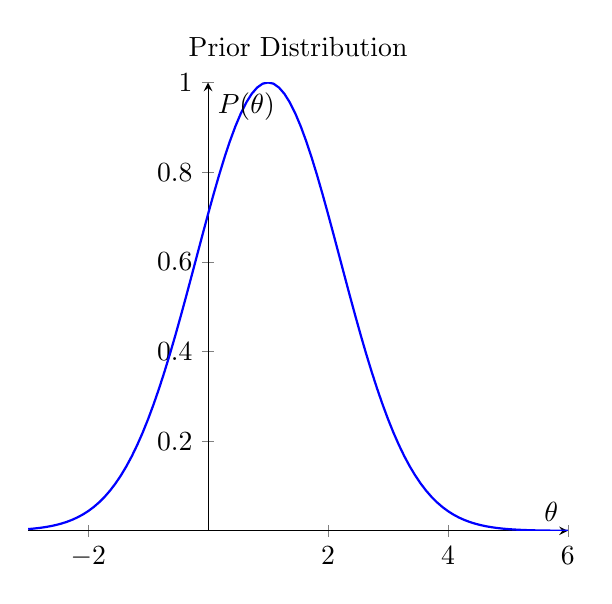
\begin{tikzpicture}
			\begin{axis}[
				domain=-3:6,
				samples=100,
				ymin=0, ymax=1,
				xlabel={$\theta$},
				ylabel={$P(\theta)$},
				title={Prior Distribution},
				axis lines=middle,
				every axis plot/.append style={thick}
				]
				\addplot[blue] {exp(-0.5*((x-1)/1.2)^2)};
			\end{axis}
		\end{tikzpicture}
	\end{subfigure}
	
	\vspace{1em} % Adds vertical spacing
	
	\begin{subfigure}{\textwidth}
		\centering
		\begin{tikzpicture}
			\begin{axis}[
				domain=-3:6,
				samples=100,
				ymin=0, ymax=1,
				xlabel={$\theta$},
				ylabel={$P(D|\theta)$},
				title={Likelihood Function},
				axis lines=middle,
				every axis plot/.append style={thick}
				]
				\addplot[green, dashed] {exp(-0.5*((x-2.5)/0.8)^2)};
			\end{axis}
		\end{tikzpicture}
	\end{subfigure}
	
	\vspace{1em} % Adds vertical spacing
	
	\begin{subfigure}{\textwidth}
		\centering
		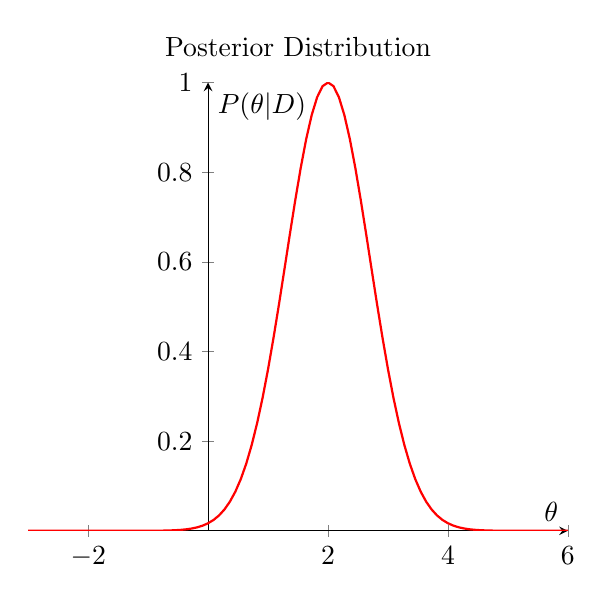
\begin{tikzpicture}
			\begin{axis}[
				domain=-3:6,
				samples=100,
				ymin=0, ymax=1,
				xlabel={$\theta$},
				ylabel={$P(\theta|D)$},
				title={Posterior Distribution},
				axis lines=middle,
				every axis plot/.append style={thick}
				]
				\addplot[red] {exp(-0.5*((x-2)/0.7)^2)};
			\end{axis}
		\end{tikzpicture}
	\end{subfigure}
	
	\caption{Bayesian updating: (Top) Prior distribution, (Middle) Likelihood function, (Bottom) Posterior distribution}
\end{figure}


\subsection{Numerical approximations for Bayesian methods}

Due to the complex nature of the likelihood function in the SEINR model, which results from integrating deterministic differential equations with stochastic observation processes, an analytical solution for the posterior distribution is not attainable. Instead, we employ numerical methods, specifically Markov Chain Monte Carlo (MCMC) techniques, to approximate the posterior.
\begin{figure}[h]
	\centering
	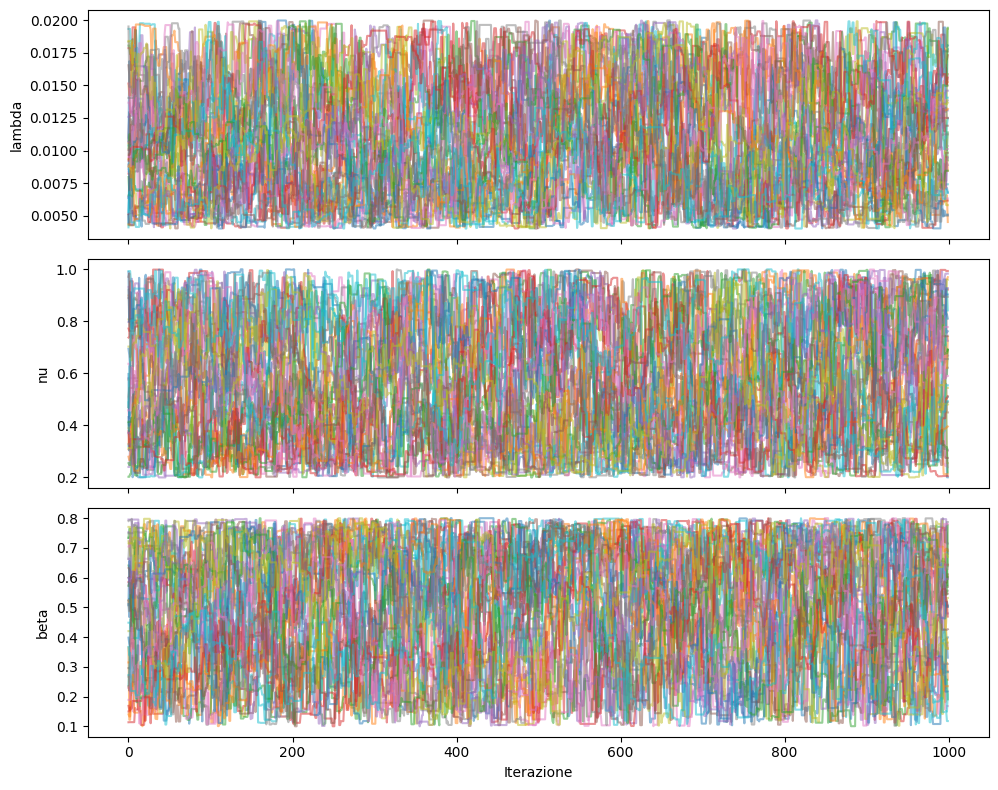
\includegraphics[width=0.7\textwidth]{Figures/markov_chain.png}  % Replace with actual figure file
	\caption{An example of MCMC chains that have explored the parameters space in its entirety (notice how dense the plots look)}
	%\label{fig:commuting_matrix}
\end{figure}
The implementation proceeds as follows:

\begin{enumerate}
	\item The parameter vector is initialized with estimates derived from existing virological literature and preliminary model calibration.
	
	\item At each iteration of the MCMC algorithm:
	\begin{itemize}
		\item A candidate set of parameters is generated using a carefully chosen proposal distribution.
		\item The candidate is then evaluated against the current parameter set by computing an acceptance probability, which depends on the ratio of their respective posterior probabilities.
	\end{itemize}
	
	\item The acceptance criterion follows the Metropolis-Hastings algorithm:
	\begin{equation}
		\alpha = \min \left( 1, \frac{P(\theta^* | D)}{P(\theta | D)} \right),
	\end{equation}
	where:
	\begin{itemize}
		\item \( \theta^* \) is the candidate parameter set,
		\item \( \theta \) is the current parameter set,
		\item \( P(\theta | D) \) is the posterior probability given the observed data \( D \).
	\end{itemize}
	If \( \theta^* \) yields a higher posterior probability, it is accepted; otherwise, it is accepted with probability \( \alpha \). This ensures that, over many iterations, the chain of sampled parameters converges to the true posterior distribution.
	
	\item Once convergence is achieved, it is assessed using diagnostic measures such as the Gelman-Rubin statistic:
	\begin{equation}
		\hat{R} = \frac{\text{Var}^+(\theta)}{W},
	\end{equation}
	where \( \text{Var}^+(\theta) \) is the pooled variance estimate and \( W \) is the within-chain variance. In our case a value of \( \hat{R} \approx 1 \) indicates convergence.
	
	\item Finally, the resulting posterior sample is used to approximate a probability distribution function, and some of its features such as average, median value and credibility intervals. 
	
	\item The approximate posterior distribution is then used in our model to make the predictions we need. In the following cycle, the posterior distribution becomes the new prior, and the numerical algorithm is triggered once again. 
\end{enumerate}

While this Bayesian approach is computationally demanding (because we need to run an enormous amount of simulations in order to approximate a continuous probability distribution), its ability to explicitly account for uncertainty and dynamically update forecasts makes it a powerful tool, particularly during periods of rapid epidemiological change (as we will see, each year has different peaks and valleys in flu incidence during the winter season).

\begin{figure}[h]
	\centering
	% First subplot: Markov Chain State Transitions
	\begin{subfigure}{0.45\textwidth}
		\centering
		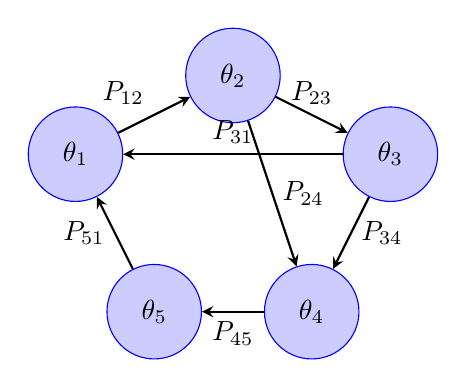
\begin{tikzpicture}
			% Nodes
			\node (S1) [state] at (0,2) {$\theta_1$};
			\node (S2) [state] at (2,3) {$\theta_2$};
			\node (S3) [state] at (4,2) {$\theta_3$};
			\node (S4) [state] at (3,0) {$\theta_4$};
			\node (S5) [state] at (1,0) {$\theta_5$};
			
			% Arrows
			\draw [arrow] (S1) -- (S2) node[midway, above left] {$P_{12}$};
			\draw [arrow] (S2) -- (S3) node[midway, above] {$P_{23}$};
			\draw [arrow] (S3) -- (S4) node[midway, right] {$P_{34}$};
			\draw [arrow] (S4) -- (S5) node[midway, below] {$P_{45}$};
			\draw [arrow] (S5) -- (S1) node[midway, left] {$P_{51}$};
			\draw [arrow] (S2) -- (S4) node[midway, right] {$P_{24}$};
			\draw [arrow] (S3) -- (S1) node[midway, above] {$P_{31}$};
		\end{tikzpicture}
		\caption{Markov Chain transitions between parameter states}
	\end{subfigure}
	\hfill
	% Second subplot: Markov Chain Monte Carlo Sampling
	\begin{subfigure}{0.45\textwidth}
		\centering
		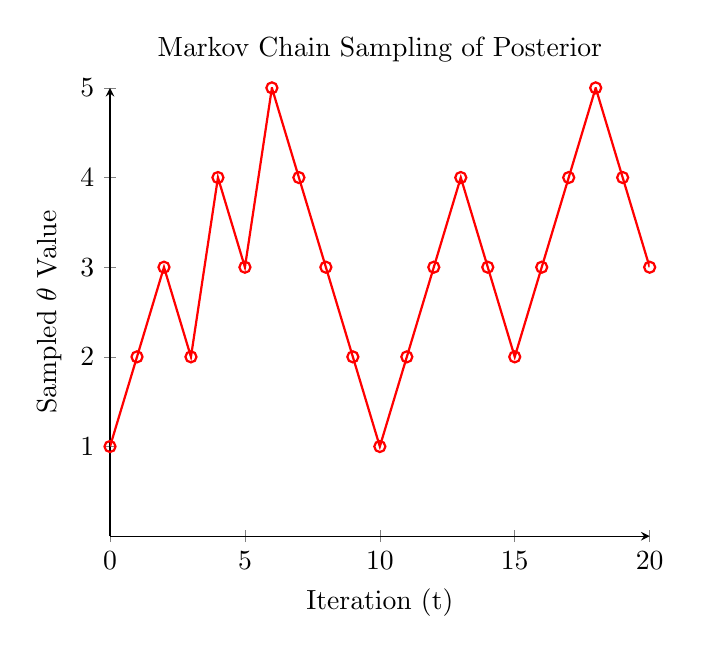
\begin{tikzpicture}
			\begin{axis}[
				domain=0:20,
				samples=100,
				xlabel={Iteration (t)},
				ylabel={Sampled $\theta$ Value},
				title={Markov Chain Sampling of Posterior},
				axis lines=left,
				ymin=0, ymax=5,
				xtick={0,5,10,15,20},
				ytick={1,2,3,4,5},
				every axis plot/.append style={thick}
				]
				% Simulated MCMC sample path
				\addplot[red, mark=o] coordinates {(0,1) (1,2) (2,3) (3,2) (4,4) (5,3) (6,5) (7,4) (8,3) (9,2) (10,1) (11,2) (12,3) (13,4) (14,3) (15,2) (16,3) (17,4) (18,5) (19,4) (20,3)};
			\end{axis}
		\end{tikzpicture}
		\caption{MCMC sampling process for Bayesian inference}
	\end{subfigure}
	
	% Third subplot: Posterior reconstruction histogram
	\begin{subfigure}{0.9\textwidth}
		\centering
		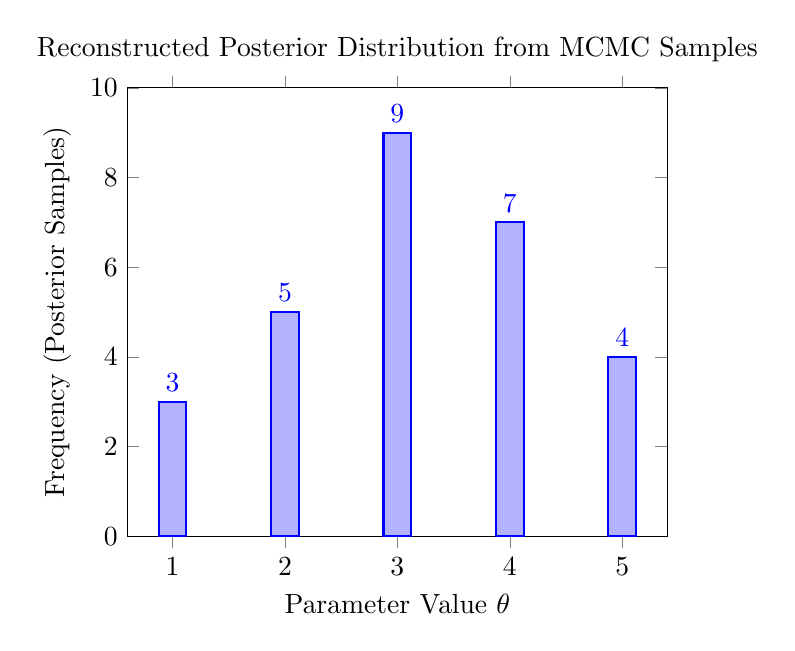
\begin{tikzpicture}
			\begin{axis}[
				ybar,
				xlabel={Parameter Value $\theta$},
				ylabel={Frequency (Posterior Samples)},
				title={Reconstructed Posterior Distribution from MCMC Samples},
				symbolic x coords={1,2,3,4,5},
				xtick=data,
				ymin=0, ymax=10,
				nodes near coords,
				every axis plot/.append style={thick, fill=blue!50}
				]
				% Simulated posterior distribution histogram
				\addplot coordinates {(1,3) (2,5) (3,9) (4,7) (5,4)};
			\end{axis}
		\end{tikzpicture}
		\caption{Histogram showing posterior probability reconstruction}
	\end{subfigure}
	
	\caption{Markov Chain in Bayesian Inference: (a) A Markov Chain transitions between different parameter states. (b) Over time, an MCMC sampler explores these states, generating samples from the posterior. (c) A histogram of these samples reconstructs the posterior probability distribution.}
\end{figure}


\chapter{Coding and Implementation}

Next, we will describe the practical aspects of implementing our SEINR model using Python. The implementation relies on a combination of high-level libraries for numerical computations, data handling, and file management. We will also describe the strategy we employed to numerically solve a time-discrete system of ODEs. 

From now on, the non-bayesian strategy of using a fixed distribution of parameters each week (without a posteriori updates) will be considered a particular case of bayesian modelling where the prior distribution is equal to the posterior: this is done to avoid confusion and for brevity's sake, since most sections of the code are similar for both strategies. 

\section{Coding Bayesian Inference}

Our approach to Bayesian inference relies on a combination of Python libraries. \textit{NumPy} is used for computationally efficient math operations and array management. For example, \texttt{np.linspace} is used to generate uniformly spaced values for parameters like the latency rate (\(\nu\)), the transmission rate (\(\lambda\)), the infectiousness period (\(\beta\)), and the recovery rate (\(\gamma\)). This allows us to explore a broad range of parameter combinations efficiently.

We rely on \textit{Pandas} for reading and manipulating CSV files containing flu incidence data. A crucial part of the code involves iterating through the available data files, extracting all relevant information (such as region names, year, week, and target values), and aggregating this data into structured dictionaries.

For instance, one section of the code reads regional CSV files, extracts the latest available data for each region, and builds a dictionary containing weekly incidence values. This ensures that the model?s input data is always based on the most recent available records.

\subsection{Solving the SEINR Model}

To numerically solve the system of ODEs, we use a discrete approach, simulating the model on a day-by-day basis. Each time step corresponds to one day, and the numerical integration method used is similar to an explicit Euler integration scheme. At each step, the state variables ()Susceptible, Exposed, Infectious, Non-infectious, and Removed) are updated according to the differential equations governing the phenomenon (which are explained in detail in chapter 1). 

\subsection{Bayesian Updates and Parameter Estimation}

For the Bayesian updates, we integrate prior parameter distributions with simulation results. The implementation follows an iterative approach:

\begin{enumerate}
	\item A large number of simulations are run for a single week using sampled parameter sets.
	\item The model outputs weekly incidence predictions, which are then compared to real incidence data using a Gaussian likelihood function.
	\item The likelihood values are used to weight the parameter sets (e.g: which parameters are more likely to cause this data?).
	\item The updated posterior is saved and used as the new prior for subsequent iterations.
\end{enumerate}

These steps are repeated each week, and each week our estimates of the parameters should become slightly more adapted to real-world data.

\section{Forecast File Format for Influcast Repository}

To contribute weekly influenza forecasts to the Influcast GitHub repository, our predictions must be formatted according to a predefined structure and saved as CSV files. Each file needs to follow a strict naming convention and contains specific columns to ensure compatibility with the system.

\subsection{File Naming and Storage}

Forecast files are stored within the repository using the following path structure:
\begin{center}
	\texttt{previsioni/Team\_X-Modello\_Y/2024\_05.csv}
\end{center}

where:
\begin{itemize}
	\item \texttt{Team\_X} represents the name of the forecasting team.
	\item \texttt{Modello\_Y} identifies the model (MetaFlu in our case) used for the predictions.
	\item \texttt{2024\_05.csv} refers to the year and  week of the forecast.
\end{itemize}

\subsection{CSV File Structure}

Each forecast file must contain the following columns:

\begin{table}[h]
	\centering
	\renewcommand{\arraystretch}{1.2}
	\begin{tabular}{|c|c|l|}
		\hline
		\textbf{Column Name} & \textbf{Type} & \textbf{Description} \\
		\hline
		\texttt{anno} & Integer & Year of the forecast. \\
		\texttt{settimana} & Integer & week of the forecast. \\
		\texttt{luogo} & String & Location code (national or regional). \\
		\texttt{tipo\_valore} & String & Always set to "quantile". \\
		\texttt{id\_valore} & Float & Quantile value (from 0.01 to 0.99). \\
		\texttt{orizzonte} & Integer & Forecast horizon (from 1 to 4). \\
		\texttt{valore} & Float & Predicted weekly incidence per 1000 patients. \\
		\texttt{target} & String & Prediction target (ILI in our case). \\
		\hline
	\end{tabular}
	\caption{Required columns for forecast CSV files.}
	\label{tab:forecast_format}
\end{table}

\subsection{Column Details}

\begin{itemize}
	\item \textbf{anno, settimana}: The year and epidemiological week of the forecast, stored as integers. These values must match those in the surveillance report and the filename (except for the leading zero in single-digit weeks).
	\item \textbf{luogo}: A two-character code indicating the forecast's geographical scope:
	\begin{itemize}
		\item \texttt{IT}: National forecast.
		\item \texttt{01} - \texttt{21}: Regional codes, following the official mapping:
		\begin{itemize}
			\item \texttt{01}: Abruzzo, \texttt{02}: Basilicata, \texttt{03}: Calabria, \dots, \texttt{21}: Veneto.
		\end{itemize}
	\end{itemize}
	\item \textbf{tipo\_valore}: This field is always set to "quantile".
	\item \textbf{id\_valore}: Represents the quantile for which the forecast is provided. Required quantiles include:
	\begin{center}
		0.01, 0.025, 0.05, 0.1, 0.15, 0.2, 0.25, 0.3, 0.35, 0.4, 0.45, 0.5, 0.55, 0.6, 0.65, 0.7, 0.75, 0.8, 0.85, 0.9, 0.95, 0.975, 0.99.
	\end{center}
	\item \textbf{orizzonte}: An integer indicating the forecast horizon:
	\begin{itemize}
		\item \texttt{-1}, \texttt{0}: the most recent and second-most recent surveillance week. Some models include these values in their output file, but they are not necessary in order to participate to the project. 
		\item \texttt{1} - \texttt{4}: Predictions for one to four weeks ahead.
	\end{itemize}
	\item \textbf{valore}: A floating-point number representing the predicted weekly incidence (cases per 1000 patients), corresponding to the given week, quantile, and location.
	\item \textbf{target}: Specifies the type of forecast. Allowed values are:
	\begin{itemize}
		\item \texttt{ILI}: Influenza-like illness.
		\item \texttt{ILI+FLU-A}: Influenza-like illness, including influenza A cases.
		\item \texttt{ILI+FLU-B}: Influenza-like illness, including influenza B cases.
	\end{itemize}
\end{itemize}

\subsection{Example of a Valid Forecast File}

Below is an excerpt from a correctly formatted CSV output file:

\begin{verbatim}
	anno,settimana,luogo,tipo_valore,id_valore,orizzonte,valore,target
	2023,45,IT,quantile,0.975,1,0.982,ILI
	2023,45,IT,quantile,0.975,2,0.995,ILI
	2023,45,IT,quantile,0.975,3,1.084,ILI
	2023,45,IT,quantile,0.975,4,1.174,ILI
	2023,45,IT,quantile,0.5,1,0.934,ILI+_FLU_A
	2023,45,IT,quantile,0.5,2,0.956,ILI+_FLU_A
\end{verbatim}

\begin{figure}[h]
	\centering
	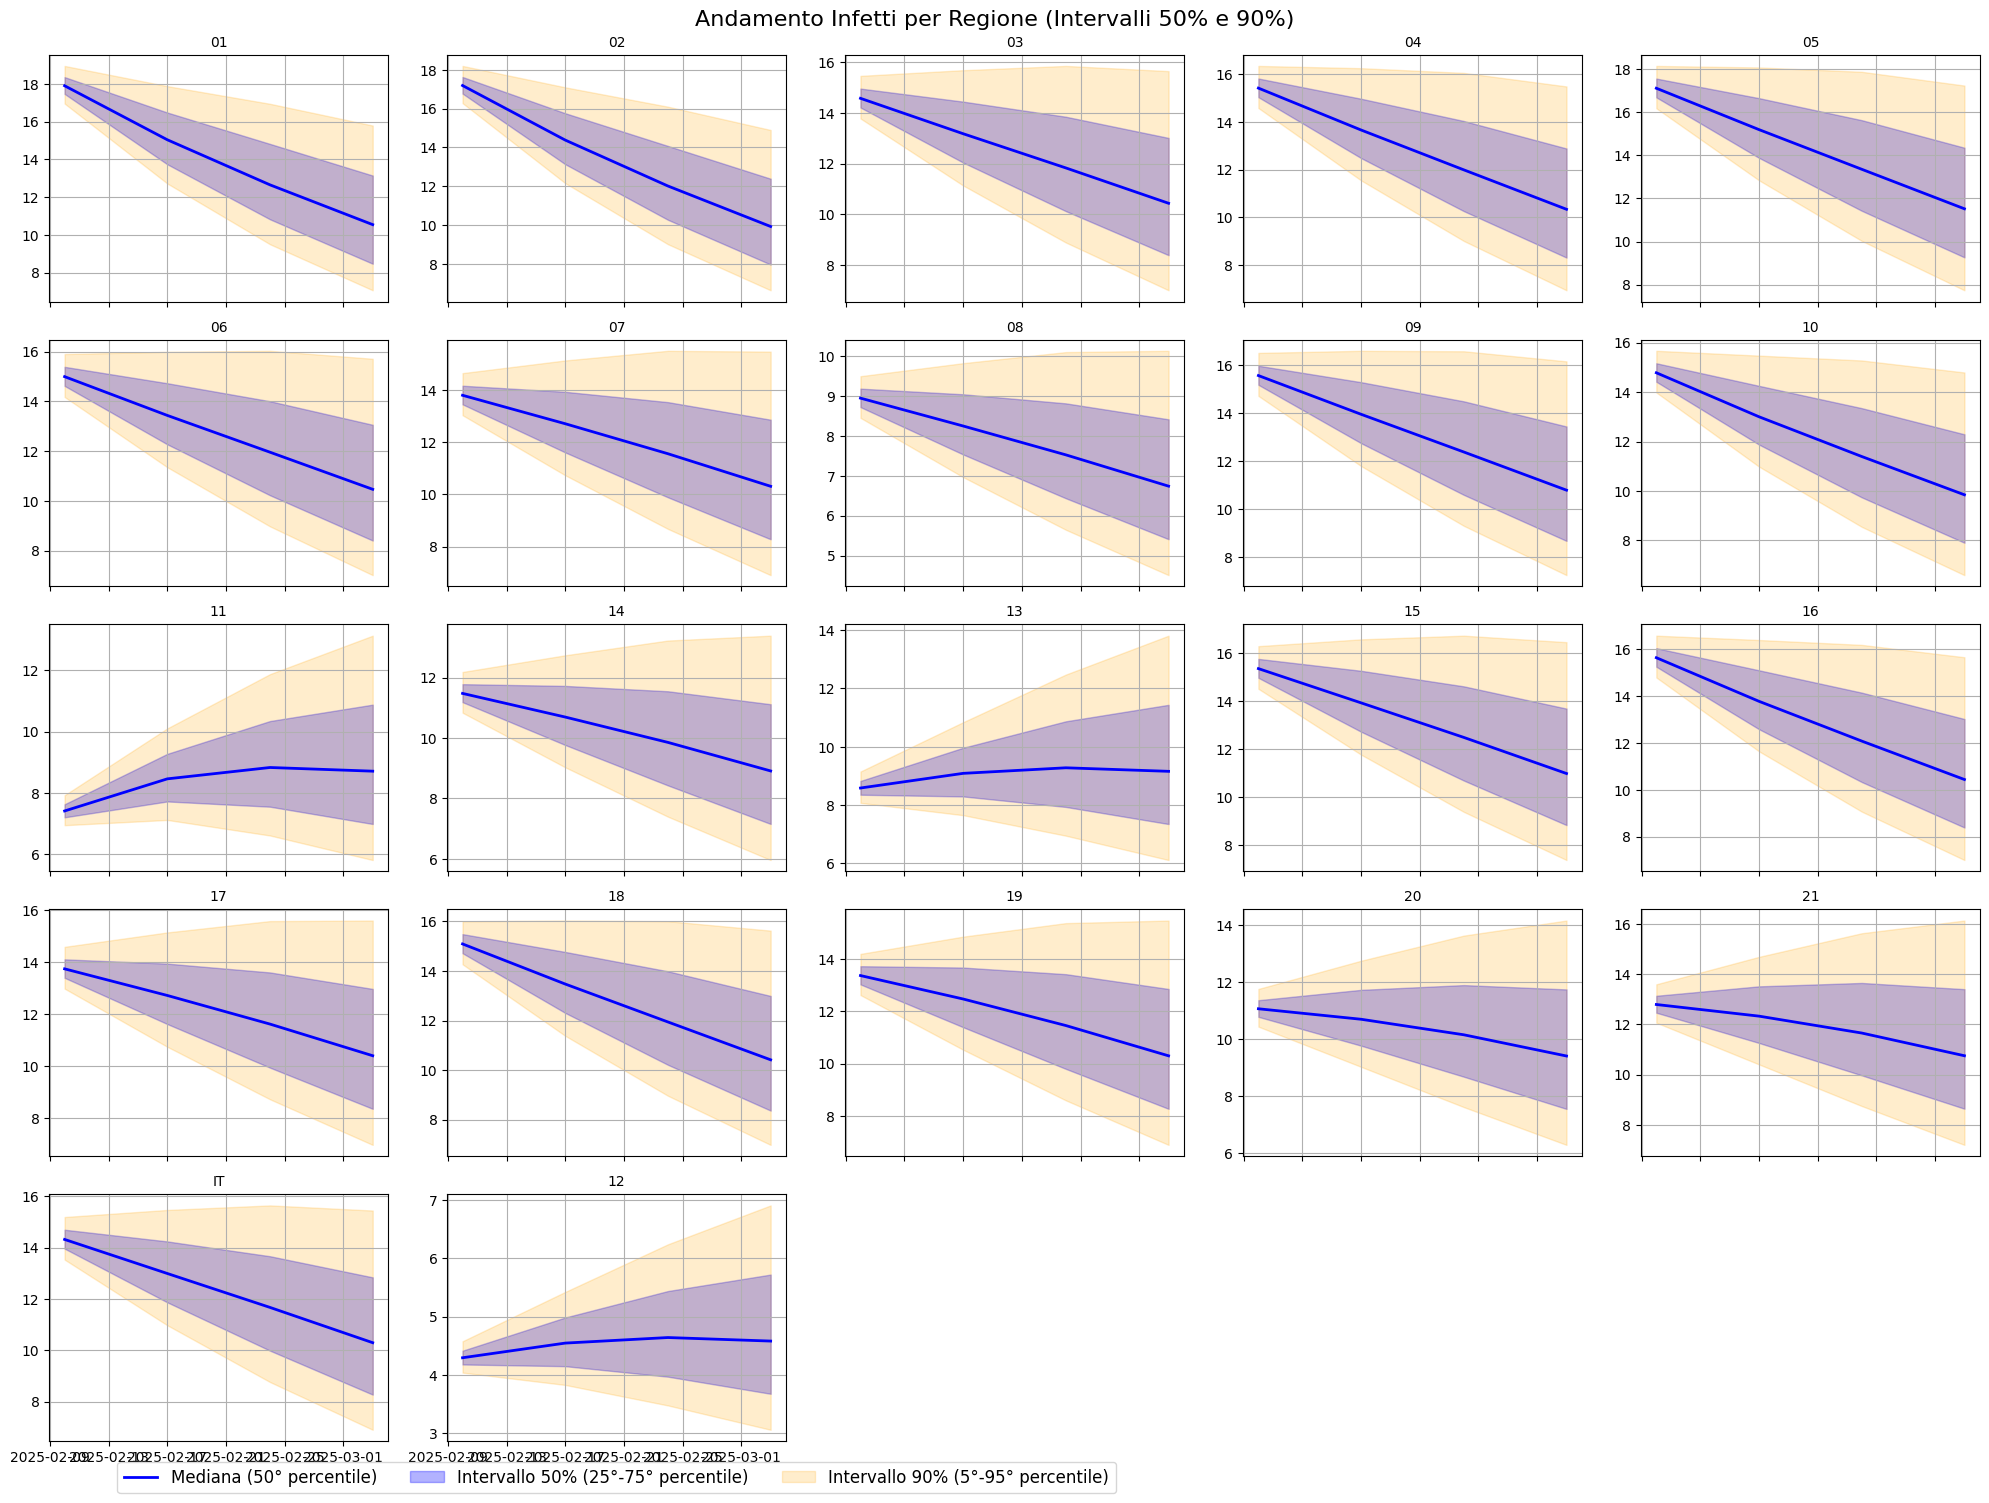
\includegraphics[width=0.7\textwidth]{Figures/influcast_output.png}  % Replace with actual figure file
	\caption{A graphical visualization of an output file uploaded to Influcast}
	%\label{fig:commuting_matrix}
\end{figure}

\chapter{Experiments and Contributions}\label{sec:cont}

As explained, the main goal of this thesis was to test whether the SEINR metapopulation model, which had worked well for COVID-19, could also capture influenza dynamics in an effective way. Along the way, I took part in several projects that served as real-world tests for the model and helped shape its development.

\section{Collaborative Projects}

\subsection{Influcast}

Influcast is Italy?s first central hub for epidemiological forecasts, gathering estimates from different research teams on influenza-like illness (ILI) trends at both national and regional levels. The project is coordinated by the ISI Foundation in Turin, and the predictions provided by each team are based on case reports from a network of sentinel doctors, with data provided every Friday by the Italian National Institute of Health (ISS) through the RespiVirNet bulletin.

It should be kept in mind that the reported ILI cases do not just reflect influenza but also include other respiratory viruses like SARS-CoV-2 and Rhinovirus. The platform updates every Wednesday, giving teams enough time to process the latest data, recalibrate their models, and publish forecasts covering the next four weeks. 

\begin{figure}[h]
	\centering
	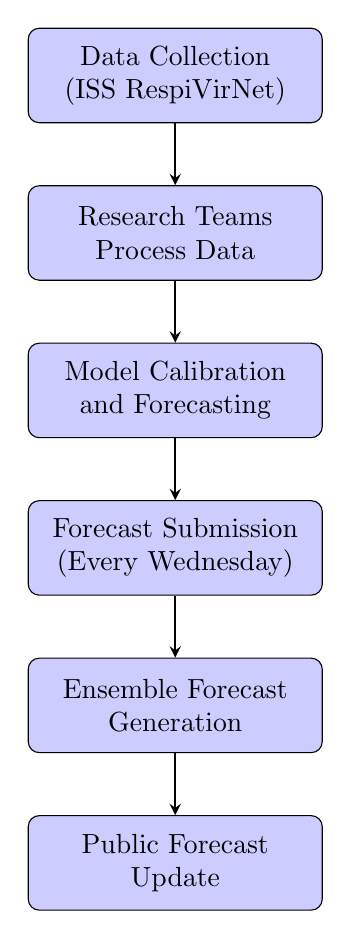
\begin{tikzpicture}[node distance=2cm]
		
		% Nodes (Using \parbox to allow line breaks)
		\node (data) [process] {\parbox{3.5cm}{\centering Data Collection \\ (ISS RespiVirNet)}};
		\node (teams) [process, below of=data] {\parbox{3.5cm}{\centering Research Teams \\ Process Data}};
		\node (models) [process, below of=teams] {\parbox{3.5cm}{\centering Model Calibration \\ and Forecasting}};
		\node (submission) [process, below of=models] {\parbox{3.5cm}{\centering Forecast Submission \\ (Every Wednesday)}};
		\node (ensemble) [process, below of=submission] {\parbox{3.5cm}{\centering Ensemble Forecast \\ Generation}};
		\node (update) [process, below of=ensemble] {\parbox{3.5cm}{\centering Public Forecast Update}};
		
		% Arrows
		\draw [arrow] (data) -- (teams);
		\draw [arrow] (teams) -- (models);
		\draw [arrow] (models) -- (submission);
		\draw [arrow] (submission) -- (ensemble);
		\draw [arrow] (ensemble) -- (update);
		
	\end{tikzpicture}
	\caption{Workflow of Influcast: Data is collected from ISS RespiVirNet, processed by research teams, forecasted models are submitted, and an ensemble forecast is generated for public updates.}
	\label{fig:influcast_workflow}
\end{figure}

\begin{figure}[h]
	\centering
	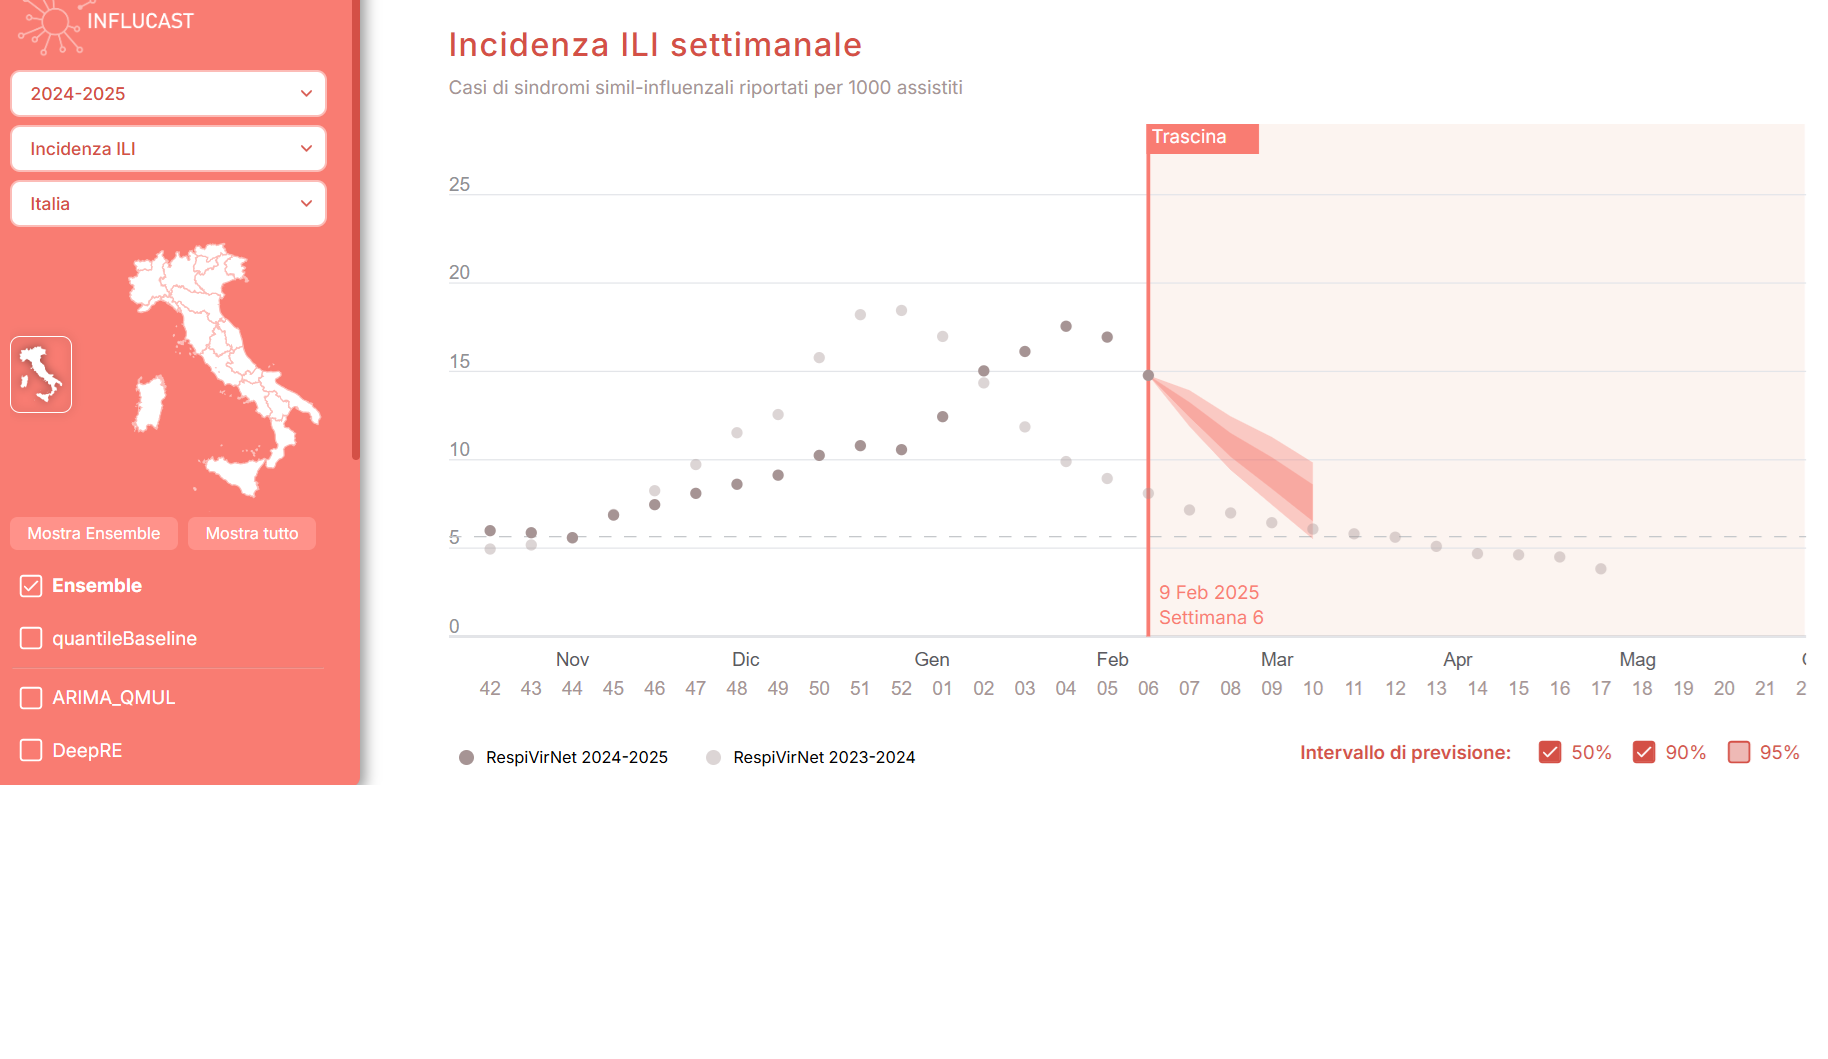
\includegraphics[width=0.7\textwidth]{Figures/influcast_front_end.png}  % Replace with actual figure file
	\caption{ Influcast front-end interface, containing past data (both 2023-2024 and 2024-2025 seasons) and forecasts for future weeks.}
	\label{fig:influcast_front_end}
\end{figure}

\subsection{Respicast}

Respicast grew out of the COVID-19 Forecasting Hub, which launched in March 2021 and quickly became an important reference point for European research teams. In November 2023, Respicast expanded to also include forecasts for other respiratory illnesses like ILI and acute respiratory infections (ARI). \cite{respicast}

Its goal is to give reliable, near-term projections to help public health officials and the general public stay ahead of outbreaks, while also building a strong open-source community of disease modelers.

\begin{figure}[h]
	\centering
	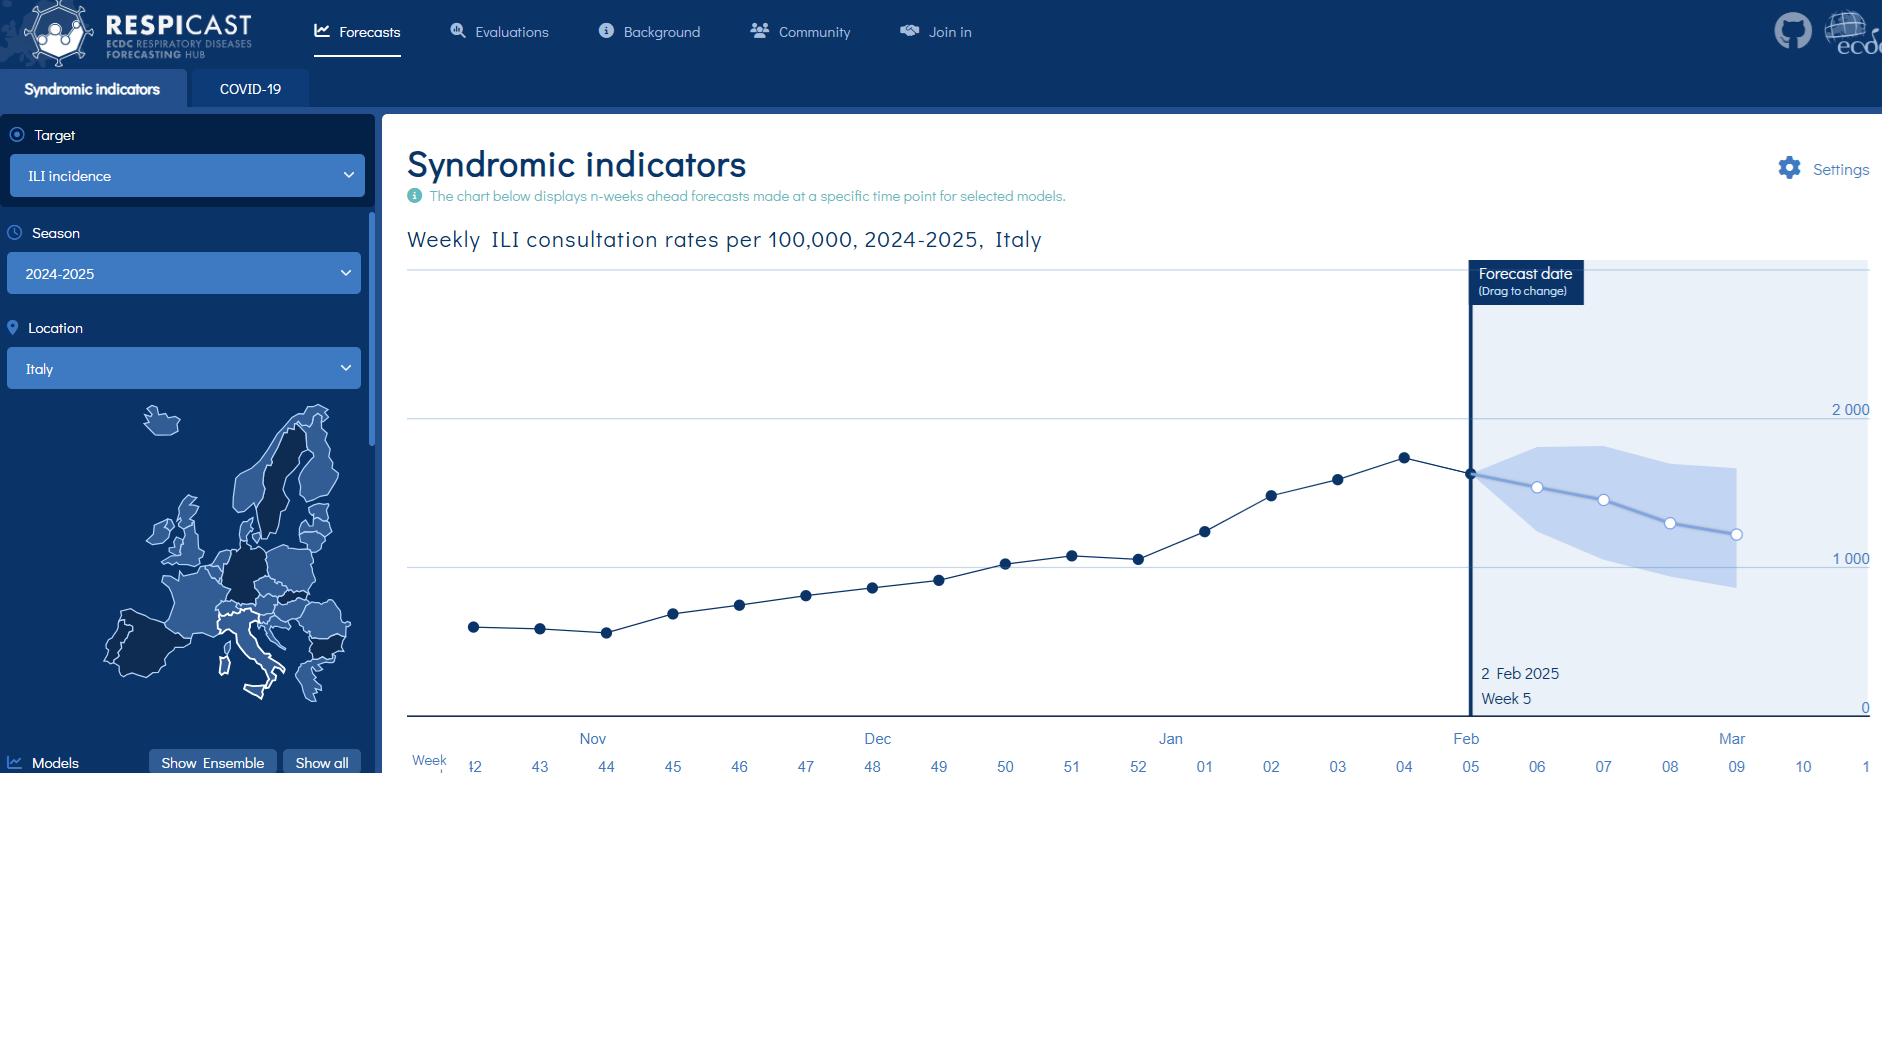
\includegraphics[width=0.7\textwidth]{Figures/respicast_front_end.png}  % Replace with actual figure file
	\caption{ Respicast front-end interface, containing past data (2024-2025 season) and forecasts for future weeks.}
	\label{fig:influcast_front_end}
\end{figure}

\section{Collaborative Paper Published}

All this work led to a collaborative paper titled \textit{?Collaborative forecasting of influenza-like illness in Italy: The Influcast experience?} \cite{influcast}. Over the 2023/2024 winter season, the project carried out 20 forecasting rounds, with five research teams contributing a total of eight different models. These forecasts, which predicted ILI incidence up to four weeks in advances, were combined into an ensemble model. 

\begin{figure}[h]
	\centering
	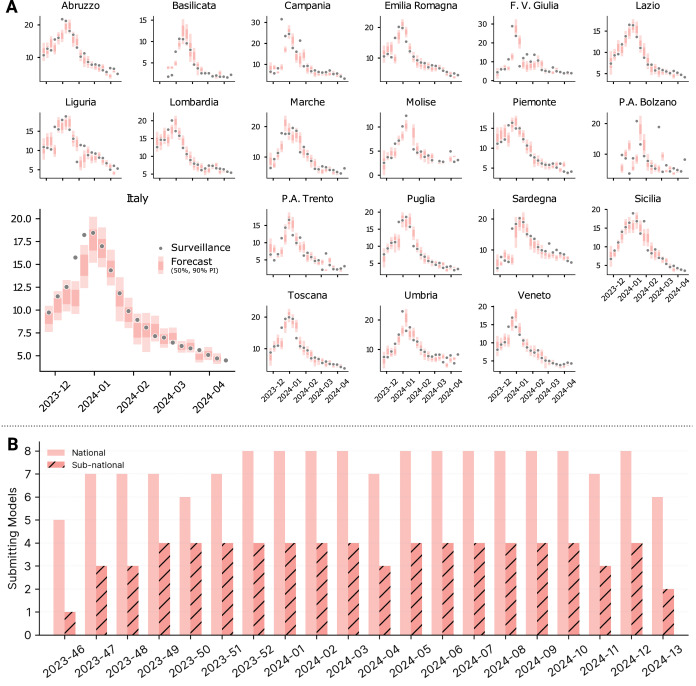
\includegraphics[width=0.7\textwidth]{Figures/influcast_models_submission.jpg}  % Replace with actual figure file
	\caption{ (A): Ensemble predictions for a 1-week horizon (with 50 percent and 90 percent confidence intervals) at the national and regional level in different submission rounds. (B) How many models submitted predictions for each submission round. Taken from \cite{influcast}}
	%\label{fig:commuting_matrix}
\end{figure}

As we will see in the section regarding model validation, the ensemble consistently ranked among the best compared to individual models and a baseline forecast. Its performance worsened slightly over longer horizons, but the ensemble still outperformed the baseline across all timeframes. 


\chapter{Model Validation}
Confronta i risultati ottenuti con i due metodi con le varie metriche di errore (log score, weighted interval score, mean relative error, mean absolute error, coverage) spiegando pregi e difetti di ognuna

\section{Christmas Holiday issue}
Parla del picco di casi a Natale e mostra che l'utilizzo di Bayes risolve parzialmente il problema, mostra che tutti i modelli di Influcast hanno fatto fatica in quel periodo
\section{Methodology}
Spiega come verificare quale dei due approcci (bayesiano e puramente deterministico) si comporta meglio nel periodo critico natalizio

\section{Numerical results}

Metti tutti i grafici e tutte le tabelle per le varie regioni con le metriche dell'errore\cite{influcast}
%\begin{figure}[tb!]
%\begin{center}
%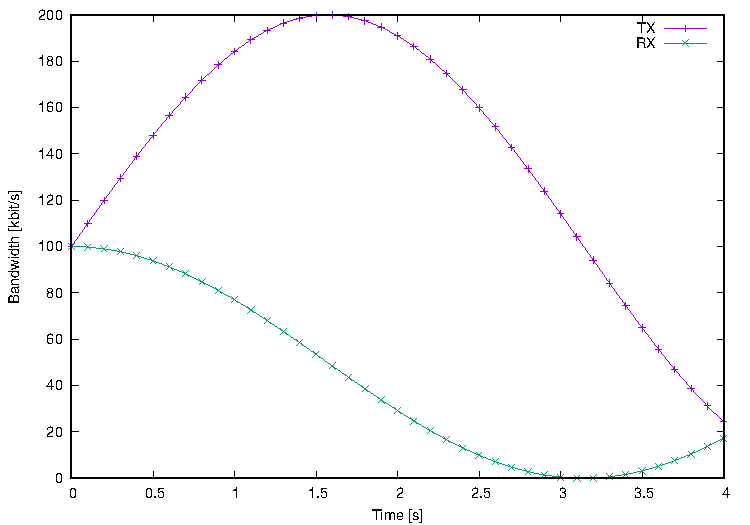
\includegraphics[width=10cm]{Figures/sino.pdf}
%\caption{grafico di esempio.}\label{fig:bw}
%\end{center}
%\end{figure}

%Some basic hints:
%\begin{itemize}
%\item both x and y axes should be properly labeled. %Units of measurements must be {\em always} reported!
%\item if the curve are experimental or by simulation, remember to report always all the points in addition to the line connecting them
%\end{itemize}

\begin{figure}[h]
	\centering
	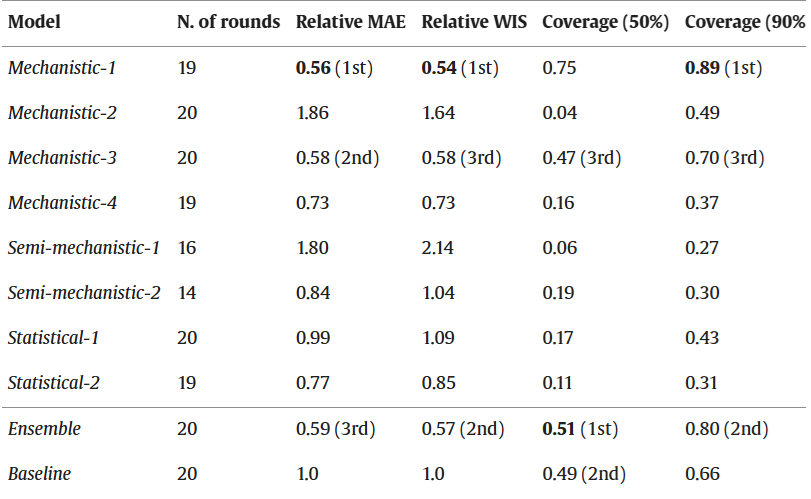
\includegraphics[width=0.7\textwidth]{Figures/influcast_paper_table.png}  % Replace with actual figure file
	\caption{ Predictive performance of each model. How different models performed in terms of relative MAE of the median, relative WIS, 50 percent and 90 percent coverage. The best model for each metric is highlighted in bold. Taken from \cite{influcast}}
	%\label{fig:commuting_matrix}
\end{figure}

\begin{figure}[h]
	\centering
	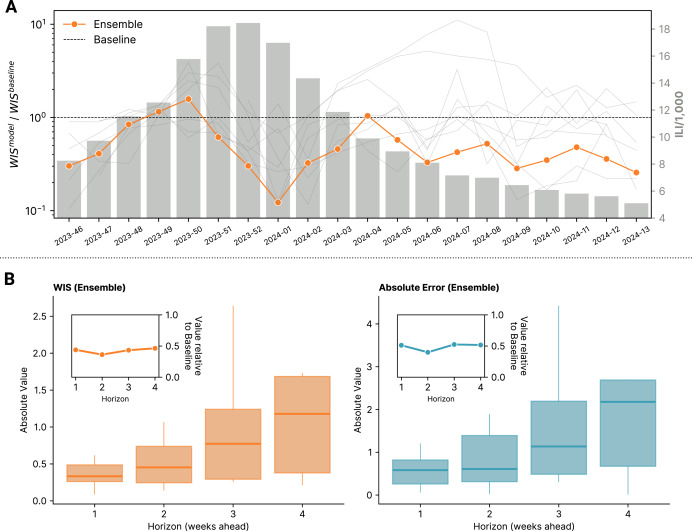
\includegraphics[width=0.7\textwidth]{Figures/influcast_paper_performance_by_horizon.jpg}  % Replace with actual figure file
	\caption{ Performance of submitted models in time and by horizon. (A) Ratio between average WIS of different models and of the baseline (both obtained averagign for 1 to 4 weeks horizons) for various forecast rounds. If a value is smaller than 1, that model performs better than baseline. The ensemble model is plotted in orange, while baseline model is the black dashed line. The vertical bars in the background show the reported incidence for that week. (B) Absolute WIS values of the Ensemble model for various horizons (from 
		to 
		weeks ahead). On the right, we repeat the analysis considering the absolute error of the median as a performance metric. The box boundaries represent the interquartile range (IQR), the line inside the box indicates the median and the whiskers extend to 1.5 times the IQR from the quartiles. Taken from \cite{influcast}}
	%\label{fig:commuting_matrix}
\end{figure}



\chapter{Conclusion}

Riporta molto brevemente che risultati abbiamo ottenuto, ricalca l'importanza dell'approccio bayesiano. 

Spiega i punti deboli del nostro modello: la struttura provinciale della matrice di pendolarismo si sposa male col fatto che i dati reali sono su base regionale. Il fatto che i dati reali vengano forniti su base settimanale influisce negativamente, dato che il modello ragiona in maniera giornaliera. Servono anche piu' dati sull'efficacia del vaccino, e l'applicabilita' del nostro modello e' limitata a singole stagioni influenzali in cui non si prevede la possibilita' di reinfezione. 

L'approccio bayesiano probabilmente migliora la precisione del modello (cio' va confermato nei prossimi anni se vogliamo esserne sicuri) ma aumenta in maniera drammatica i costi computazionali, e se si vuole ovviare a questo problema e' necessario applicare l'inferenza bayesiana a pochissimi parametri. Menziona brevemente la questione underfitting e overfitting, e chiedersi se includere il compartimento N comporti dei guadagni in accuratezza. 

Proponi spunti per espandere il modello e implementare stime meno onerose per i parametri con il machine learning o l'intelligenza artificiale

\bibliographystyle{plain}
\bibliography{biblio}

\end{document}
